\documentclass{ieeeaccess}

\usepackage{spotcolor}

% Bold font setup for ieeeaccess
\makeatletter
\AtBeginDocument{\DeclareMathVersion{bold}
\SetSymbolFont{operators}{bold}{T1}{times}{b}{n}
\SetSymbolFont{NewLetters}{bold}{T1}{times}{b}{it}
\SetMathAlphabet{\mathrm}{bold}{T1}{times}{b}{n}
\SetMathAlphabet{\mathit}{bold}{T1}{times}{b}{it}
\SetMathAlphabet{\mathbf}{bold}{T1}{times}{b}{n}
\SetMathAlphabet{\mathtt}{bold}{OT1}{pcr}{b}{n}
\SetSymbolFont{symbols}{bold}{OMS}{cmsy}{b}{n}
\renewcommand\boldmath{\@nomath\boldmath\mathversion{bold}}}
\makeatother

\def\BibTeX{{\rm B\kern-.05em{\sc i\kern-.025em b}\kern-.08em
    T\kern-.1667em\lower.7ex\hbox{E}\kern-.125emX}}

\usepackage[utf8]{inputenc}
\usepackage{booktabs}
\usepackage{graphicx}
\usepackage{subcaption}
\usepackage{amsmath}
\usepackage{amssymb}
\usepackage{multirow}
\usepackage{url}
\usepackage{cite}
\usepackage{float}
\usepackage{tabularx}
\usepackage{array}

% Custom command definitions
\newcommand{\at}[1]{@#1}

\begin{document}
\history{Date of publication August 01, 2026, date of current version August 01, 2026.}
\doi{10.1109/ACCESS.2026.0429000}

% ==============================================================================
% TITLE & AUTHORS
% ==============================================================================
\title{A Multi-Criteria Benchmark of Collaborative Filtering Paradigms for Scientific Paper Recommendation: A Study of Robustness and Generalization}

\author{\uppercase{Xavier Peña}\authorrefmark{1},
AND \uppercase{Diego Rivera}\authorrefmark{2}}
\address[1]{Carrera de Computación, Facultad de Ingeniería, Universidad de Cuenca, Cuenca 010150, Ecuador (e-mail: xavier.pena@ucuenca.edu.ec)}
\address[2]{Universidad Politécnica Salesiana, Cuenca 010105, Ecuador (e-mail: driverag2@est.ups.edu.ec)}
\tfootnote{Both authors contributed equally to this work. D. Rivera is also Vice-President of the IEEE Vehicular Technology Society (VTS) Ecuador Chapter.}
\corresp{Corresponding author: Xavier Peña (e-mail: xavier.pena@ucuenca.edu.ec).}

\markboth
{Peña and Rivera: A Multi-Criteria Benchmark of Collaborative Filtering Paradigms}
{Peña and Rivera: A Multi-Criteria Benchmark of Collaborative Filtering Paradigms}



% ==============================================================================
% ABSTRACT
% ==============================================================================
\begin{abstract}
The rapid growth of scientific literature makes it challenging for researchers to discover relevant articles. While implicit collaborative filtering (CF) is a standard approach, existing evaluations are often fragmented, ignoring engineering trade-offs or statistical validation across multiple domains. This article addresses these gaps through a multi-criteria, multidimensional benchmark of six representative recommender paradigms (memory-based, deep neural networks, graph neural networks, and Transformers). The models are evaluated under a unified protocol combining time-ordered Leave-One-Out (LOO) and Random Split (RS) schemes on three real-world datasets: CiteULike-a, CiteULike-t, and BibSonomy (36 independent experimental conditions). Our analysis goes beyond ranking accuracy (Recall, Normalized Discounted Cumulative Gain [NDCG], Mean Reciprocal Rank [MRR]) to assess catalog coverage, Gini index, popularity bias, computational costs (GPU memory, throughput), and sensitivity to training data reduction (50\% and 20\% downsampling, inducing cold-start noise). The ranking results analyzed via the Friedman test ($\chi^2 = 26.00, p < 0.001$, Kendall's $W = 0.8667$) and post-hoc Nemenyi test ($\alpha=0.05$) reveal that no single paradigm dominates all dimensions. While MultiVAE and NeuMF achieve the highest accuracy in larger datasets, they exhibit severe popularity bias and high sensitivity to data reduction. Conversely, LightGCN and SASRec demonstrate lower combined sensitivity to data scarcity and cold-start. ItemKNN requires zero training overhead while delivering the highest diversity, serving as a highly competitive baseline for resource-constrained environments. All source code, configs, and preprocessed datasets are publicly available.
\end{abstract}

\begin{keywords}
Recommender systems, scientific literature, collaborative filtering, graph neural networks, Transformers, robustness, statistical analysis.
\end{keywords}

\titlepgskip=-21pt
\maketitle

% ==============================================================================
% 1. INTRODUCTION
% ==============================================================================
\section{Introduction}
The volume of scientific and technical publications continues to grow, overwhelming traditional academic dissemination channels. This information overload poses an operational challenge for researchers and students, who must spend considerable time identifying relevant works for their lines of research. In this context, scientific literature recommender systems (SR) offer a solution to personalize the discovery flow of articles based on users' previous interactions.

The predominant scenario in academic paper recommendation is \emph{collaborative filtering with implicit feedback}. Unlike commercial environments with explicit ratings (such as 1 to 5 star ratings), the signal available in reference managers or social bookmarking platforms consists of binary events (such as saving an article to a personal folder, downloading it, or reading it). Mathematically modeling this implicit signal presents two main challenges: first, there is no direct negative feedback, as the absence of interaction does not necessarily imply disinterest, but rather lack of awareness of the article; second, the user-item interaction matrix exhibits extreme sparsity, with densities frequently falling below 0.5\%.

To address these challenges, the machine learning community has proposed various model families:
\begin{itemize}
    \item \textbf{ItemKNN:} Represents the heuristic memory-based approach~\cite{sarwar2001item}. It computes statistical co-occurrence similarities over the interaction columns without requiring trainable parameters, serving as an efficiency control.
    \item \textbf{NeuMF (Neural Matrix Factorization):} Combines generalized matrix factorization with deep feed-forward networks~\cite{he2017neural}, replacing the traditional inner product with learned non-linear representations.
    \item \textbf{MultiVAE:} Models the user's interaction history as a sample coming from a latent multinomial distribution using a variational autoencoder~\cite{liang2018variational}.
    \item \textbf{SASRec and BERT4Rec:} Utilize self-attention mechanisms (Transformers), unidirectional~\cite{kang2018self} and bidirectional~\cite{sun2019bert4rec} respectively, assuming sequential reading dynamics.
    \item \textbf{LightGCN:} Simplifies propagation over the user-item bipartite graph by removing non-linear weight transformations and activations~\cite{he2020lightgcn}, performing embedding aggregations over neighboring nodes.
\end{itemize}

Despite the rapid development of these architectures, recent studies point out that offline experimental evaluations in the field tend to focus solely on ranking accuracy (such as NDCG\at{10}), omitting reproducibility analysis or systematic comparisons against well-tuned heuristic baselines, as argued by Dacrema et al.~\cite{dacrema2019really} and Petrov and Macdonald~\cite{petrov2023effective}. Furthermore, engineering aspects such as memory footprint, inference throughput, or performance degradation under data scarcity are rarely integrated into a unified evaluation framework.

To address these limitations, this study presents a multi-dimensional comparative analysis of the six model families over three independent datasets (CiteULike-a, CiteULike-t, and BibSonomy). The study addresses four primary research questions:

\begin{itemize}
    \item \textbf{RQ1 (Accuracy vs. Complexity):} Do deep learning-based models show a statistically significant increase in ranking accuracy compared to well-tuned heuristic baselines?
    \item \textbf{RQ2 (Consistency across Collections):} Do model performance rankings remain consistent when evaluated on collections with different densities and interaction volumes?
    \item \textbf{RQ3 (Sensitivity to Data Reduction):} To what extent does each model's accuracy degrade when training data is reduced to 50\% and 20\% while keeping the evaluation set constant?
    \item \textbf{RQ4 (Multi-Criteria Trade-offs):} Is there a single dominant algorithm across all evaluated dimensions, or are there trade-offs between accuracy, diversity, resilience, and computational cost?
\end{itemize}

% ==============================================================================
% 2. STATE OF THE ART AND RELATED WORK
% ==============================================================================
\section{State of the Art and Related Work}
\label{sec:related_work}

Scientific literature recommendation has evolved from systems based on natural language processing and content-based filtering (Content-Based Filtering) to collaborative approaches based on latent representations. This section examines the three fundamental lines in which this research is framed.

\subsection{Implicit Collaborative Filtering in Academic Literature}
Unlike commercial domains where platforms like Netflix or Amazon have explicit ratings or frequent clicks, the academic domain is characterized by implicit interactions of low frequency but high thematic specificity. Hu et al.~\cite{hu2008collaborative} and Koren et al.~\cite{koren2009matrix} formalized implicit matrix factorization models (WRMF) by assigning confidence weights to observed interactions. However, linear techniques suffer from intrinsic limitations to capture non-linear co-citation patterns or interdisciplinary research dynamics.

\subsection{Evolution towards Deep Neural Architectures}
The introduction of Neural Collaborative Filtering (NeuMF) by He et al.~\cite{he2017neural} showed that traditional dot products could be complemented by multilayer perceptrons (MLP). Subsequently, Liang et al.~\cite{liang2018variational} proposed MultiVAE, suggesting that the multinomial loss function outperforms binary cross-entropy when modeling the competitive nature of item selection in a large catalog.

In the sequential domain, Kang and McAuley introduced SASRec~\cite{kang2018self}, adapting the causal self-attention of Transformers to capture users' reading trajectories. Sun et al. extended this concept with BERT4Rec~\cite{sun2019bert4rec}, applying the bidirectional Cloze model. More recently, He et al. proposed LightGCN~\cite{he2020lightgcn}, observing that in collaborative filtering over bipartite graphs, the non-linear weight transformations of traditional GCNs are redundant and can degrade performance.

\subsection{Reproducibility Crisis and Recent Multi-Criteria Evaluation}
Despite the theoretical advance proposed by each of these families, works like that of Dacrema et al.~\cite{dacrema2019really} and Petrov and Macdonald~\cite{petrov2023effective} revealed that a considerable proportion of recent neural methods fail to outperform simple heuristic algorithms (such as ItemKNN or UserKNN) when the latter are calibrated rigorously. Additionally, Krichene and Rendle~\cite{krichene2020sampled} exposed how sampled metrics impose methodological biases on offline comparisons. Recent studies by Yuan et al.~\cite{yuan2023benchmarking} and Ferraro et al.~\cite{ferraro2024fairness} highlight the need to evaluate recommenders under multidimensional criteria that integrate catalog coverage, Gini index, and computational costs. The present work responds to these recommendations by evaluating six models under a non-sampled protocol and over multiple engineering axes.

% ==============================================================================
% 3. MATHEMATICAL FORMULATION OF PARADIGMS
% ==============================================================================
\section{Formulation of Recommender Paradigms}
\label{sec:paradigms}

With the purpose of formalizing the operational bases of each algorithm, their detailed mathematical formulations, loss functions, and optimization targets are presented below.

\subsection{Memory-Based Collaborative Filtering (ItemKNN)}
The ItemKNN algorithm~\cite{sarwar2001item} estimates preferences from statistical similarity over the implicit interaction matrix $R \in \{0, 1\}^{|U| \times |I|}$. The adjusted cosine similarity between item $i$ and item $j$, adjusted by a regularization or smoothing parameter (shrinkage) $h \ge 0$, is expressed as:
\begin{equation}
S_{ij} = \frac{|U_i \cap U_j|}{\sqrt{|U_i| \cdot |U_j|} + h}
\end{equation}
where $U_i = \{u \in U : R_{ui} = 1\}$ represents the set of users who have interacted with item $i$. The parameter $h$ attenuates similarity values inflated by pairs of items with very few interactions.

The predicted score $\hat{y}_{ui}$ for user $u$ on item $i$ is obtained by weighting the similarities of $i$ with the set of items in the user's history $H_u = \{j \in I : R_{uj} = 1\}$, considering only the $k$ nearest neighbors $S^k(i)$:
\begin{equation}
\hat{y}_{ui} = \sum_{j \in S^k(i) \cap H_u} S_{ij}
\end{equation}

\subsection{Neural Matrix Factorization (NeuMF)}
The NeuMF model~\cite{he2017neural} integrates a Generalized Matrix Factorization (GMF) component and a Multi-Layer Perceptron (MLP) in parallel. The GMF component computes the element-wise product of user and item embeddings:
\begin{equation}
\phi^{GMF} = \mathbf{p}_u^G \odot \mathbf{q}_i^G
\end{equation}
The MLP component processes the concatenation of user and item embeddings through $L$ non-linear hidden layers:
\begin{equation}
\phi_1^{MLP} = a_1(\mathbf{W}_1^T [\mathbf{p}_u^M \parallel \mathbf{q}_i^M] + \mathbf{b}_1)
\end{equation}
\begin{equation}
\phi_L^{MLP} = a_L(\mathbf{W}_L^T \phi_{L-1}^{MLP} + \mathbf{b}_L)
\end{equation}
where $a_L$ represents the ReLU activation function. The final prediction layer concatenates the resulting vectors and applies a sigmoid function:
\begin{equation}
\hat{y}_{ui} = \sigma(\mathbf{h}^T [\phi^{GMF} \parallel \phi_L^{MLP}])
\end{equation}
The optimization is performed by minimizing the binary cross-entropy (BCE) loss function over a set of observed interactions $Y$ and negative samples $Y^-$:
\begin{equation}
\mathcal{L}_{BCE} = -\sum_{(u, i) \in Y \cup Y^-} y_{ui} \log \hat{y}_{ui} + (1 - y_{ui}) \log (1 - \hat{y}_{ui})
\end{equation}

\subsection{Variational Autoencoder for Collaborative Filtering (MultiVAE)}
MultiVAE~\cite{liang2018variational} adopts a probabilistic generative approach. It assumes that for each user $u$, a latent representation $\mathbf{z}_u \sim \mathcal{N}(0, \mathbf{I}_K)$ is generated. The binary interaction vector $\mathbf{x}_u \in \{0, 1\}^{|I|}$ is modeled as a sample from a multinomial distribution conditioned on $\mathbf{z}_u$:
\begin{equation}
\mathbf{x}_u \sim \text{Mult}(N_u, \pi(\mathbf{z}_u)), \quad \pi(\mathbf{z}_u) = \text{softmax}(f_\theta(\mathbf{z}_u))
\end{equation}
where $f_\theta$ represents the decoder network parameterized by $\theta$. The variational encoder network $g_\phi(\mathbf{x}_u)$ approximates the posterior distribution:
\begin{equation}
q_\phi(\mathbf{z}_u | \mathbf{x}_u) = \mathcal{N}(\mu_\phi(\mathbf{x}_u), \text{diag}(\sigma_\phi^2(\mathbf{x}_u)))
\end{equation}
The learning objective consists in maximizing the Evidence Lower Bound (ELBO) regularized by an annealing factor $\beta \in [0, 1]$:
\begin{equation}
\mathcal{L}_u(\theta, \phi) = \mathbb{E}_{q_\phi(\mathbf{z}_u | \mathbf{x}_u)}[\log p_\theta(\mathbf{x}_u | \mathbf{z}_u)] - \beta \cdot D_{KL}(q_\phi(\mathbf{z}_u | \mathbf{x}_u) \parallel p(\mathbf{z}_u))
\end{equation}

\subsection{Self-Attentive Sequential Recommendation (SASRec)}
SASRec~\cite{kang2018self} processes ordered interaction sequences $S_u = (s_1, s_2, \dots, s_t)$. To preserve chronology, it combines item embeddings with a trainable positional embedding $\mathbf{P} \in \mathbb{R}^{N \times d}$:
\begin{equation}
\mathbf{E} = [\mathbf{e}_{s_1} + \mathbf{p}_1; \mathbf{e}_{s_2} + \mathbf{p}_2; \dots; \mathbf{e}_{s_t} + \mathbf{p}_t]
\end{equation}
The matrix $\mathbf{E}$ is projected into Queries ($\mathbf{Q}$), Keys ($\mathbf{K}$), and Values ($\mathbf{V}$):
\begin{equation}
\mathbf{Q} = \mathbf{E}\mathbf{W}_Q, \quad \mathbf{K} = \mathbf{E}\mathbf{W}_K, \quad \mathbf{V} = \mathbf{E}\mathbf{W}_V
\end{equation}
Self-attention is computed by applying a causal mask $\mathbf{M}$ ($M_{ij} = -\infty$ for $i < j$, and $0$ otherwise):
\begin{equation}
\text{Attention}(\mathbf{Q}, \mathbf{K}, \mathbf{V}) = \text{softmax}\left(\frac{\mathbf{Q} \mathbf{K}^T}{\sqrt{d}} + \mathbf{M}\right) \mathbf{V}
\end{equation}
The output passes through point-wise feed-forward networks with residual connections and layer normalization (Layer Normalization).

\subsection{Bidirectional Sequential Recommendation (BERT4Rec)}
BERT4Rec~\cite{sun2019bert4rec} extends sequential analysis using bidirectional Transformer attention. During training, the Cloze objective is applied by randomly replacing $p\%$ of the items in the sequence with a special token \texttt{[mask]}:
\begin{equation}
s'_i = \begin{cases} \text{\texttt{[mask]}}, & \text{with probability } p \\ s_i, & \text{with probability } 1-p \end{cases}
\end{equation}
Unlike SASRec, BERT4Rec does not use a causal mask $\mathbf{M}$, allowing each position to attend to both left and right context. The model is trained by maximizing the log-likelihood of the masked items:
\begin{equation}
\mathcal{L} = -\sum_{s_i \in S_u^{mask}} \log P(s_i | S'_u)
\end{equation}

\subsection{Simplified Graph Convolution (LightGCN)}
LightGCN~\cite{he2020lightgcn} performs information propagation over the user-item bipartite graph. In each layer $k+1$, the representation of a node is obtained by aggregating the embeddings of its neighbors weighted by the degree of the nodes:
\begin{equation}
\mathbf{e}_u^{(k+1)} = \sum\limits_{i \in N_u} \frac{1}{\sqrt{|N_u| \cdot |N_i|}} \mathbf{e}_i^{(k)}
\end{equation}
\begin{equation}
\mathbf{e}_i^{(k+1)} = \sum\limits_{u \in N_i} \frac{1}{\sqrt{|N_i| \cdot |N_u|}} \mathbf{e}_u^{(k)}
\end{equation}
After $K$ layers of propagation, the embeddings of each level are linearly averaged:
\begin{equation}
\mathbf{e}_u = \sum\limits_{k=0}^K \frac{1}{K+1} \mathbf{e}_u^{(k)}, \quad \mathbf{e}_i = \sum\limits_{k=0}^K \frac{1}{K+1} \mathbf{e}_i^{(k)}
\end{equation}
The user $u$'s preference for item $i$ is estimated as the dot product $\hat{y}_{ui} = \mathbf{e}_u^T \mathbf{e}_i$, optimized using the Bayesian Personalized Ranking (BPR) loss regularized by the $L_2$ norm:
\begin{equation}
\mathcal{L}_{BPR} = -\sum\limits_{u \in U} \sum\limits_{i \in N_u} \sum\limits_{j \notin N_u} \log \sigma(\hat{y}_{ui} - \hat{y}_{uj}) + \lambda \Vert \mathbf{E}^{(0)} \Vert^2
\end{equation}

% ==============================================================================
% 4. EXPERIMENTAL METHODOLOGY AND COMPUTATIONAL ENVIRONMENT
% ==============================================================================
\section{Experimental Methodology and Computational Environment}
\label{sec:methodology}

Figure~\ref{fig:pipeline} illustrates the methodological scheme of the study, covering from data acquisition and filtering to statistical tests.

\begin{figure}[t]
\centering
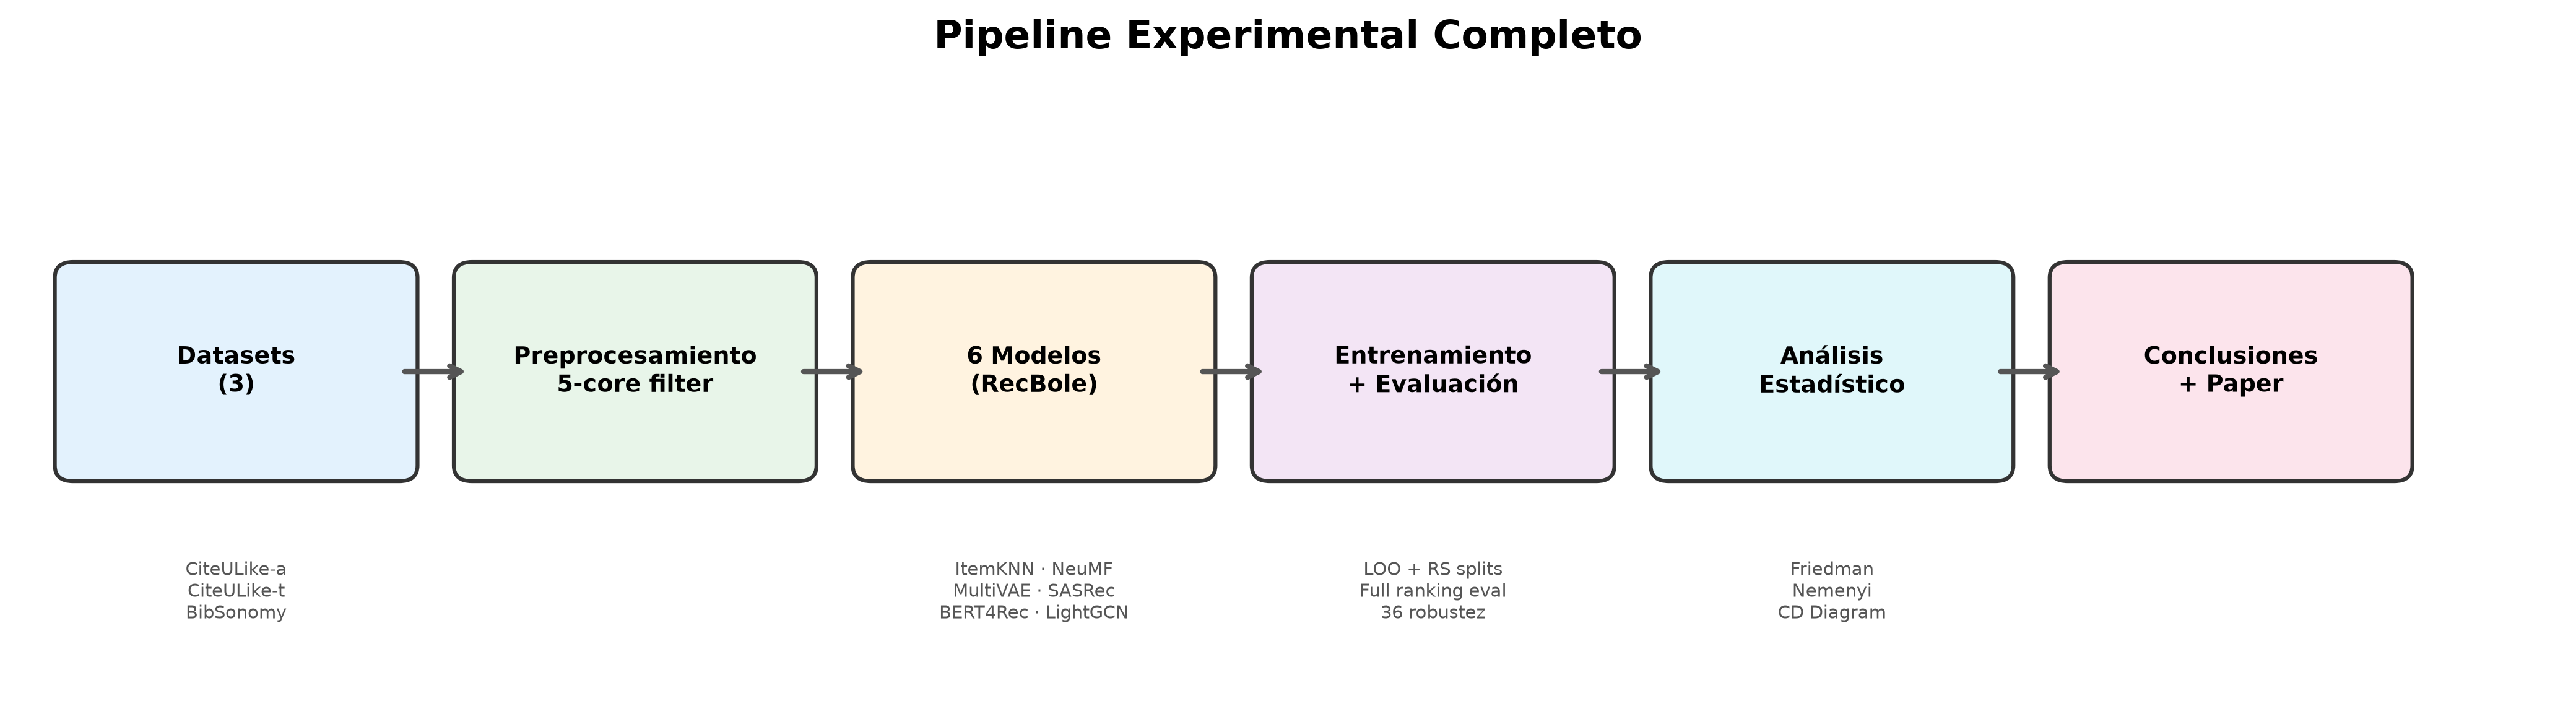
\includegraphics[width=0.48\textwidth]{figures/fig1_pipeline.png}
\caption{Scheme of the evaluation methodological flow.}
\label{fig:pipeline}
\end{figure}

\subsection{Theoretical Justification of Evaluated Paradigms and Models}
The selection of the six architectures responds to criteria of theoretical coverage in the implicit collaborative filtering literature:
\begin{itemize}
    \item \textbf{ItemKNN (Memory-Based Filtering):} Included as a non-parametric comparison point~\cite{sarwar2001item}. Its presence allows verifying the observations of Dacrema et al.~\cite{dacrema2019really} regarding the competitiveness of simple statistical methods against neural models.
    \item \textbf{NeuMF (Neural Matrix Factorization):} Represents the transition from linear models to combinations with dense feed-forward networks~\cite{he2017neural}.
    \item \textbf{MultiVAE (Probabilistic Generative Model):} Evaluated for its variational modeling approach under multinomial distributions~\cite{liang2018variational}, oriented to capture preferences over wide catalogs.
    \item \textbf{SASRec (Causal Sequential Self-Attention):} Incorporated to examine whether the sequence of past interactions provides predictive information in reading patterns~\cite{kang2018self}.
    \item \textbf{BERT4Rec (Bidirectional Sequential Self-Attention):} Selected to contrast the effect of bidirectional self-attention against strict causal schemes~\cite{sun2019bert4rec}.
    \item \textbf{LightGCN (Bipartite Graph Learning):} Represents the state of the art in graph convolution networks applied to recommendation~\cite{he2020lightgcn}, evaluating the impact of neighbor aggregation in bipartite structures.
\end{itemize}

\subsection{Dataset Selection}
To evaluate the generalization of the observations, three real-world and independent datasets were selected:
\begin{itemize}
    \item \textbf{CiteULike-a and CiteULike-t:} Come from the CiteULike platform and exhibit differences in scale and number of items per user. CiteULike-a includes title and abstract metadata (\texttt{citeulike-a.item}) useful for content inspection tasks.
    \item \textbf{BibSonomy:} Independent collection coming from the social bookmarking system of the University of Kassel, allowing evaluation of model behavior under a small-scale and high relative density (2.4284\%) data distribution. Under the LOO protocol, the test set contains exactly 325 interactions (one per user), which implies high variance in ranking metrics for this dataset; under RS, the 10\% test split assigns on average $\sim$3.9 items per user.
\end{itemize}

Table~\ref{tab:datasets} summarizes the quantitative characteristics of each collection after applying the filtering protocol.

\begin{table}[h]
\centering
\caption{Structural properties of datasets (post 5-core filtering).}
\label{tab:datasets}
\begin{tabular}{lrrrrr}
\toprule
\textbf{Dataset} & \textbf{Users} & \textbf{Items} & \textbf{Interactions} & \textbf{Density} & \textbf{Int./User} \\
\midrule
CiteULike-a & 5,536 & 15,429 & 200,180 & 0.2344\% & 36.16 \\
CiteULike-t & 3,527 & 6,339  & 77,546  & 0.3468\% & 21.99 \\
BibSonomy   & 325   & 1,607  & 12,683  & 2.4284\% & 39.02  \\
\bottomrule
\end{tabular}
\end{table}

Figure~\ref{fig:dataset_stats} presents the comparative distribution of these volume and density metrics.

\begin{figure}[h]
\centering
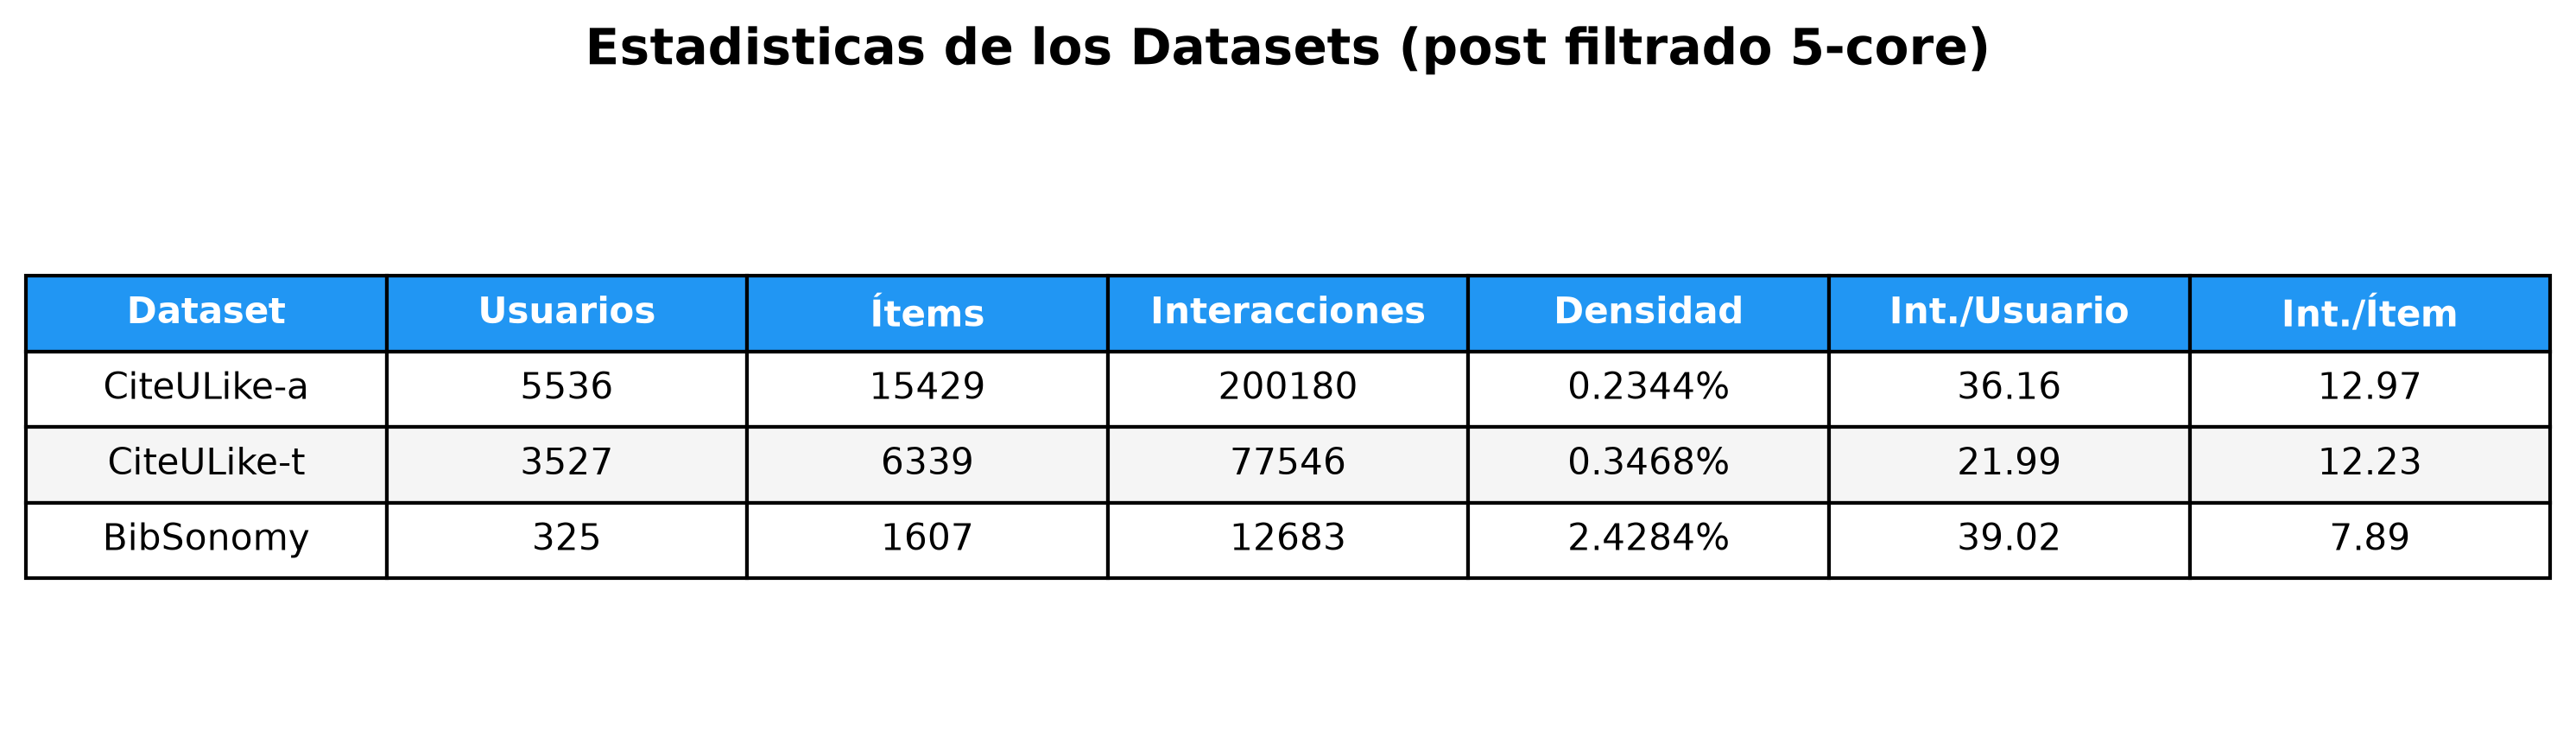
\includegraphics[width=0.45\textwidth]{figures/fig9_dataset_stats.png}
\caption{Comparative statistics of the datasets.}
\label{fig:dataset_stats}
\end{figure}

\subsection{Evaluation Protocols and Preprocessing}
An iterative 5-core filtering was applied to eliminate users and items with fewer than 5 interactions, reducing the presence of sporadic records or those with insufficient signal for pure collaborative filtering.

Following the methodological recommendations of Krichene and Rendle~\cite{krichene2020sampled}, the evaluation was performed in Full Catalog Ranking mode (\texttt{mode: full} in RecBole), ranking the target item over the entire catalog (e.g., all 15,429 active items in CiteULike-a) without relying on negative sampling (\texttt{uni100}) which would artificially inflate the metrics.

To guarantee rigor and comparability with previous literature, two complementary evaluation protocols were adopted on each dataset:
\begin{enumerate}
    \item \textbf{Leave-One-Out (LOO):} Reserves the last interacted item of each user for the test set and the second-to-last for validation (exactly 1 test item per user). It strictly preserves the temporal order of interactions, being the primary and appropriate evaluation framework for sequential models (SASRec and BERT4Rec) according to Petrov and Macdonald~\cite{petrov2023effective}.
    \item \textbf{Random Split (RS 80/10/10):} Random partition stratified by user (80\% training, 10\% validation, 10\% test). In users with high activity (average of 36.16 interactions in CiteULike-a), the 10\% test split assigns on average $\sim$3.7 relevant items per user, allowing evaluation of general static collaborative preference retrieval.
\end{enumerate}

The combination of 6 models, 3 datasets, and 2 protocols generates a total of 36 independent experimental conditions.

For the robustness experiment against data scarcity (RQ3), the 50\% and 20\% subsets were generated by sampling interactions over the training set without re-applying iterative 5-core filtering at runtime.

\subsection{Hardware Specification, Batch Configuration, and Environment}
To guarantee full reproducibility of the benchmark, all runs were performed on a dedicated workstation with the following specifications:
\begin{itemize}
    \item \textbf{Graphics Processing Unit (GPU):} NVIDIA GeForce RTX 3050 Laptop GPU (4 GB GDDR6 of Video Random Access Memory (VRAM), CUDA Compute Capability 8.6).
    \item \textbf{Central Processing Unit (CPU):} AMD Ryzen 7 5800H (8 physical cores, 16 logical threads @ 3.2 GHz base, 4.4 GHz Boost).
    \item \textbf{System RAM:} 16 GB DDR4 @ 3200 MHz.
    \item \textbf{Software Environment:} Windows 11 Home / WSL2 Ubuntu 22.04 LTS, Python 3.10.12, PyTorch v2.1.2+cu121, RecBole v1.2.0~\cite{zhao2021recbole}.
\end{itemize}

All runs maintained a fixed global random seed ($\text{seed} = 2024$) specified in the base configuration file (`configs/base.yaml`). During the offline inference and evaluation phase, GPU-based models (MultiVAE, NeuMF, LightGCN, SASRec, and BERT4Rec) were executed with a uniform batch size of $B=4096$ users. Meanwhile, ItemKNN was executed in sequential matrix CPU mode.

\subsection{Theoretical Justification and Hyperparameter Configuration}
The hyperparameters of the algorithms were selected following the theoretical and empirical justifications reported in their original publications and the optimized configurations of the RecBole framework~\cite{zhao2021recbole}. Specifically, we set the number of neighbors $k=100$ and smoothing $h=10$ for ItemKNN~\cite{sarwar2001item}, MLP layers $[64, 32, 16]$ for NeuMF~\cite{he2017neural}, latent dimension $k=64$ and annealing factor $\beta=0.2$ for MultiVAE~\cite{liang2018variational}, maximum sequence length $L=50$ and $H=2$ attention heads for SASRec~\cite{kang2018self} and BERT4Rec~\cite{sun2019bert4rec}, and propagation of $K=3$ layers in LightGCN~\cite{he2020lightgcn}. Note that the total number of trainable parameters in MultiVAE (18,647,958 in CiteULike-a) scales proportionally to the dimension of the filtered input/output catalog ($|I| = 15,429$ active items after 5-core filtering, resulting in a dimension of 15,430 including the padding token required by PyTorch/RecBole), since the outer linear layer of the encoder and decoder projects over all items. It is noted that, unlike deep models that feature adaptive early stopping (patience of 10 epochs), ItemKNN hyperparameters ($k=100$, $h=10$) were adopted in a fixed manner without dataset-specific tuning, representing a baseline calibration asymmetry (see threat in Section~\ref{subsec:itemknn-tuning}).

Table~\ref{tab:hyperparams} details the architecture parameters, optimizer (Adam with LR $= 1e-3$), and early stopping criteria (patience of 10 epochs) for each model.

\begin{table}[h]
\centering
\caption{Bibliographic justification and hyperparameter settings for each evaluated model in RecBole.}
\label{tab:hyperparams}
\footnotesize
\setlength{\tabcolsep}{2.5pt}
\begin{tabular}{lp{5.5cm}}
\toprule
\textbf{Model} & \textbf{Hyperparameter Settings and Authoritative Reference} \\
\midrule
ItemKNN  & Neighbors $k=100$, smoothing $h=10$, cosine similarity~\cite{sarwar2001item}. No gradient training. \\
NeuMF    & Embedding $d=64$, MLP layers $[64, 32, 16]$, Adam, LR $= 1e-3$, max 300 epochs (patience $= 10$)~\cite{he2017neural}. \\
MultiVAE & Latent dim $k=64$, hidden $[600]$, annealing $\beta=0.2$, Adam, LR $= 1e-3$, max 300 epochs (patience $= 10$)~\cite{liang2018variational}. \\
SASRec   & Embedding $d=64$, max seq $L=50$, heads $H=2$, layers $N=2$, dropout $= 0.2$, Adam, LR $= 1e-3$, max 300 epochs (patience $= 10$)~\cite{kang2018self}. \\
BERT4Rec & Embedding $d=64$, max seq $L=50$, mask $p=0.2$, heads $H=2$, layers $N=2$, Adam, LR $= 1e-3$, max 300 epochs (patience $= 10$)~\cite{sun2019bert4rec}. \\
LightGCN & Embedding $d=64$, layers $K=3$, $\lambda=1e-4$, Adam, LR $= 1e-3$, max 300 epochs (patience $= 10$)~\cite{he2020lightgcn}. \\
\bottomrule
\end{tabular}
\end{table}

\subsection{Statistical Analysis Protocol (Without Pseudo-replication)}
To avoid the statistical pseudo-replication criticized by Demšar~\cite{demsar2006statistical}, statistical tests were designed using the $N=6$ well-defined independent experimental conditions (3 datasets $\times$ 2 partition protocols LOO and RS) as observation blocks. The non-parametric Friedman test ($\alpha = 0.05$) was applied over the ranking accuracy measurements (NDCG\at{10}) to evaluate significant global differences between the algorithms. The global effect size was quantified using Kendall's $W$ concordance:
\begin{equation}
W = \frac{\chi^2}{N(k - 1)}
\end{equation}
where $\chi^2$ is the Friedman statistic and $k=6$ is the number of models. For pairwise comparisons, the post-hoc Nemenyi test ($\alpha = 0.05$)~\cite{demsar2006statistical} was selected, determining the critical difference (CD) threshold to establish statistically significant differences between recommenders.

% ==============================================================================
% 5. EXPERIMENTAL RESULTS AND MULTI-CRITERIA BENCHMARK
% ==============================================================================
\section{Experimental Results and Multi-Criteria Benchmark}
\label{sec:results}

\subsection{Offline Ranking Accuracy across Paradigms (RQ1 and RQ2)}
Tables~\ref{tab:results-loo} and~\ref{tab:results-rs} summarize the empirical performance of the six evaluated models under the **36 independent experimental conditions** (3 datasets $\times$ 2 partition protocols $\times$ 6 architectures).

\begin{table*}[t]
\centering
\caption{Empirical ranking performance under the Leave-One-Out (LOO) protocol on the three datasets (CiteULike-a, CiteULike-t, and BibSonomy). Best values per column are in bold.}
\label{tab:results-loo}
\footnotesize
\setlength{\tabcolsep}{3.5pt}
\begin{tabular}{lccccccccc}
\toprule
& \multicolumn{3}{c}{\textbf{CiteULike-a (LOO)}} & \multicolumn{3}{c}{\textbf{CiteULike-t (LOO)}} & \multicolumn{3}{c}{\textbf{BibSonomy (LOO)}} \\
\cmidrule(lr){2-4} \cmidrule(lr){5-7} \cmidrule(lr){8-10}
\textbf{Model} & \textbf{Recall\at{10}} & \textbf{NDCG\at{10}} & \textbf{MRR\at{10}} & \textbf{Recall\at{10}} & \textbf{NDCG\at{10}} & \textbf{MRR\at{10}} & \textbf{Recall\at{10}} & \textbf{NDCG\at{10}} & \textbf{MRR\at{10}} \\
\midrule
MultiVAE & \textbf{0.8143} & \textbf{0.6912} & \textbf{0.6522} & 0.3538 & 0.2209 & 0.1801 & \textbf{0.3477} & \textbf{0.2318} & \textbf{0.1963} \\
NeuMF    & 0.4722 & 0.2611 & 0.1970 & \textbf{0.6274} & \textbf{0.4012} & \textbf{0.3311} & 0.2431 & 0.1598 & 0.1340 \\
ItemKNN  & 0.2289 & 0.1481 & 0.1235 & 0.1849 & 0.1052 & 0.0808 & 0.1200 & 0.0798 & 0.0676 \\
SASRec   & 0.2321 & 0.1239 & 0.0908 & 0.2030 & 0.1200 & 0.0944 & 0.2185 & 0.1192 & 0.0897 \\
LightGCN & 0.2115 & 0.1213 & 0.0939 & 0.0964 & 0.0521 & 0.0386 & 0.1508 & 0.0954 & 0.0785 \\
BERT4Rec & 0.0952 & 0.0459 & 0.0311 & 0.0437 & 0.0266 & 0.0214 & 0.0154 & 0.0111 & 0.0097 \\
\bottomrule
\end{tabular}
\end{table*}

\begin{table*}[t]
\centering
\caption{Empirical ranking performance under the Random Split (RS 80/10/10) protocol on the three datasets (CiteULike-a, CiteULike-t, and BibSonomy). Best values per column are in bold.}
\label{tab:results-rs}
\footnotesize
\setlength{\tabcolsep}{3.5pt}
\begin{tabular}{lccccccccc}
\toprule
& \multicolumn{3}{c}{\textbf{CiteULike-a (Random Split)}} & \multicolumn{3}{c}{\textbf{CiteULike-t (Random Split)}} & \multicolumn{3}{c}{\textbf{BibSonomy (Random Split)}} \\
\cmidrule(lr){2-4} \cmidrule(lr){5-7} \cmidrule(lr){8-10}
\textbf{Model} & \textbf{Recall\at{10}} & \textbf{NDCG\at{10}} & \textbf{MRR\at{10}} & \textbf{Recall\at{10}} & \textbf{NDCG\at{10}} & \textbf{MRR\at{10}} & \textbf{Recall\at{10}} & \textbf{NDCG\at{10}} & \textbf{MRR\at{10}} \\
\midrule
MultiVAE & \textbf{0.7159} & \textbf{0.6619} & \textbf{0.7112} & 0.2676 & 0.1830 & 0.1887 & 0.2273 & 0.1978 & 0.2491 \\
NeuMF    & 0.6216 & 0.4411 & 0.4293 & \textbf{0.5096} & \textbf{0.3445} & \textbf{0.3244} & \textbf{0.3552} & \textbf{0.2860} & \textbf{0.3282} \\
ItemKNN  & 0.2163 & 0.1740 & 0.2145 & 0.1643 & 0.1017 & 0.1045 & 0.1170 & 0.0946 & 0.1099 \\
LightGCN & 0.1979 & 0.1407 & 0.1698 & 0.0909 & 0.0566 & 0.0558 & 0.1501 & 0.1205 & 0.1424 \\
SASRec   & 0.2053 & 0.1072 & 0.0769 & 0.0825 & 0.0460 & 0.0350 & 0.1636 & 0.0930 & 0.0713 \\
BERT4Rec & 0.0829 & 0.0426 & 0.0304 & 0.0173 & 0.0092 & 0.0068 & 0.0243 & 0.0104 & 0.0064 \\
\bottomrule
\end{tabular}
\end{table*}

The empirical analysis of Tables~\ref{tab:results-loo} and~\ref{tab:results-rs} reveals the following central trends:
\begin{enumerate}
    \item \textbf{Sequential Evaluation in LOO (Temporal Preservation):} SASRec reaches its best relative performance under the Leave-One-Out protocol (Recall\at{10} = 0.2321 in CiteULike-a, 0.2030 in CiteULike-t, and 0.2185 in BibSonomy), outperforming ItemKNN and LightGCN. This confirms that causal self-attention modeling benefits from strict preservation of the reading sequence.
    \item \textbf{Medium-Scale Collections (CiteULike-a):} MultiVAE achieves the highest ranking precision in LOO (Recall\at{10} = 0.8143, NDCG\at{10} = 0.6912) and in RS (Recall\at{10} = 0.7159, NDCG\at{10} = 0.6619), followed by NeuMF. Variational multinomial loss in VAE demonstrates superior capacity to reconstruct the latent distribution when sufficient interaction volume exists.
    \item \textbf{Moderate and Dense Collections (CiteULike-t and BibSonomy):} NeuMF leads the ranking in CiteULike-t (NDCG\at{10} = 0.4012 in LOO and 0.3445 in RS) and BibSonomy under RS (NDCG\at{10} = 0.2860). However, in BibSonomy the winner inverts between protocols: MultiVAE leads in LOO (NDCG\at{10} = 0.2318) while NeuMF dominates in RS (NDCG\at{10} = 0.2860). This inversion is attributable to the small scale of the collection (325 users, LOO test set of only 325 interactions), which amplifies ranking sensitivity to the partition scheme.
    \item \textbf{Competitiveness of ItemKNN against BERT4Rec:} ItemKNN systematically outperforms BERT4Rec in NDCG\at{10} across all datasets and protocols (e.g., 0.1481 vs. 0.0459 in CiteULike-a LOO and 0.1017 vs. 0.0092 in CiteULike-t RS). These data support the observation of Dacrema et al.~\cite{dacrema2019really}, confirming that bidirectional Transformers suffer from severe overfitting and optimization problems in sparse academic implicit interaction matrices.
\end{enumerate}

These divergences in ranking ordering also manifest in the complementarity and overlap of recommendations (see Jaccard similarity analysis in Section V-E).

\subsection{Statistical Significance Tests (Friedman and Nemenyi)}
The Friedman test applied over the NDCG\at{10} measurements in the $N=6$ independent conditions yielded a statistic of $\chi^2 = 26.00$ ($df = 5, p < 0.001$), rejecting the null hypothesis of global equivalence in ranking accuracy. The obtained Kendall's concordance is $W = 0.8667$, which confirms a high degree of relative agreement between the different collections and partitions.

Figure~\ref{fig:cd} presents the Critical Difference (CD) diagram derived from Nemenyi ($\alpha = 0.05, CD = 3.08$).

\begin{figure}[h]
\centering
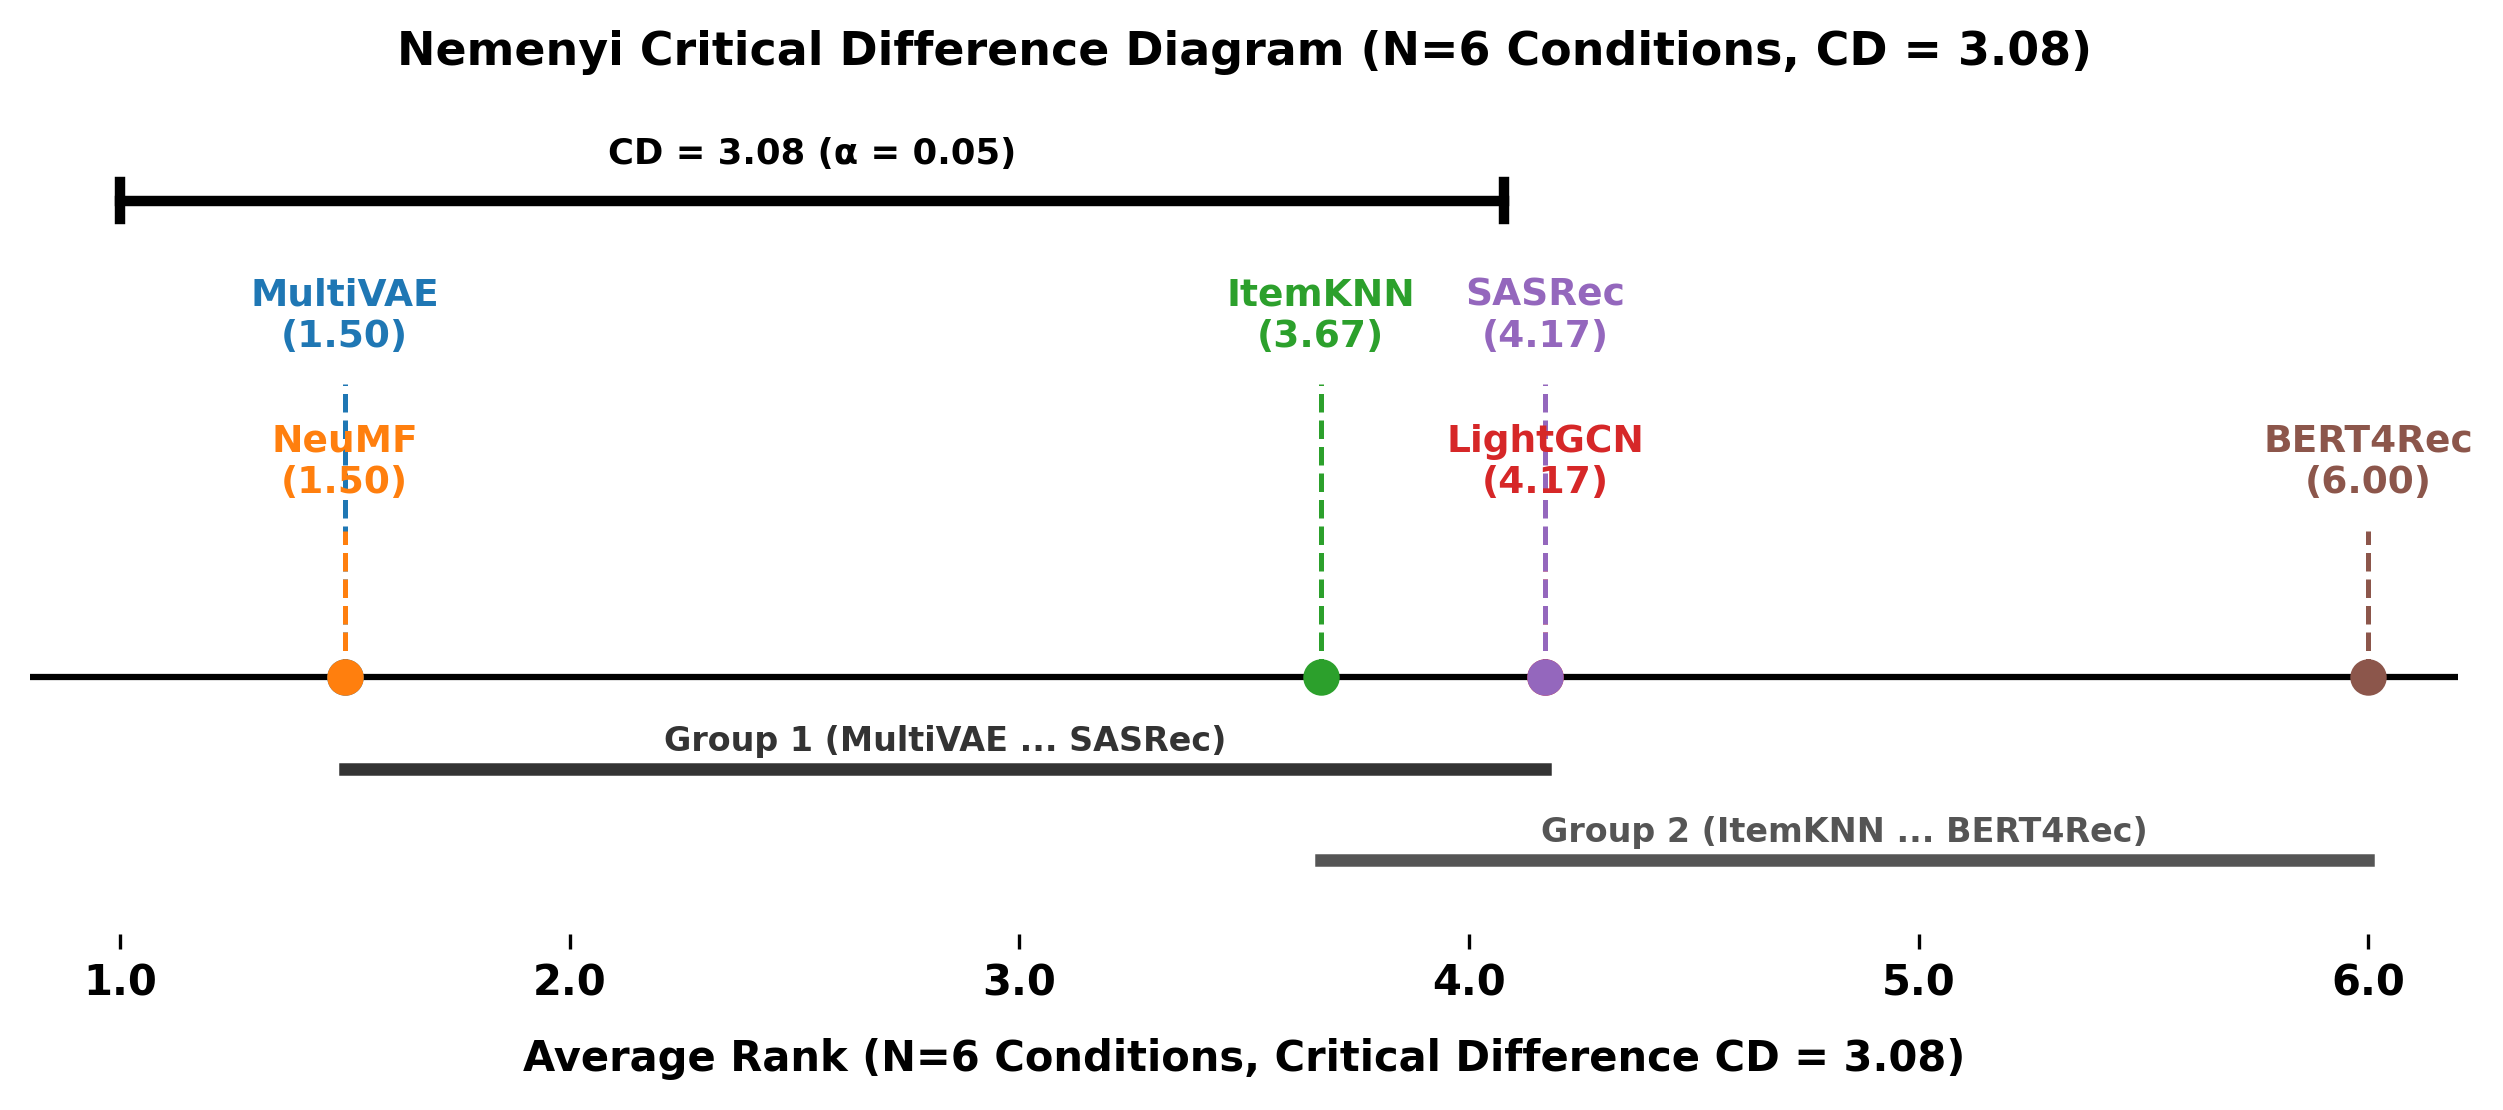
\includegraphics[width=0.45\textwidth]{figures/cd_diagram.png}
\caption{Critical Difference (CD) diagram of Nemenyi ($\alpha=0.05, CD=3.08$) over $N=6$ independent conditions.}
\label{fig:cd}
\end{figure}

The Nemenyi diagram positions MultiVAE and NeuMF at the top of the global average ranking (average rank of 1.50 both), followed by ItemKNN (3.67), LightGCN (4.17), SASRec (4.17), and BERT4Rec (6.00). Due to the limitation in the number of independent blocks ($N=6$, required to avoid statistical pseudo-replication), the Nemenyi test possesses a relatively bounded statistical power ($CD = 3.08$ with $q_{0.05} = 2.850, k=6, N=6$). Under this rigorous criterion, the only comparison that demonstrates a statistically significant superiority is that of the leading recommenders MultiVAE and NeuMF against the bidirectional Transformer BERT4Rec, since their rank difference ($4.50$) exceeds the $CD$ threshold. The remaining differences, including the dispute between deep recommenders and the linear memory baseline ItemKNN, are not statistically significant, remaining linked by the CD diagram bars. Note that, by not averaging results over multiple independent random seeds, these orderings and significances must be interpreted with caution, as they are exposed to initialization and dropout variability (i.e., the reported formal significance might be partially confounded with the stochastic variance of the single selected seed).

\subsection{Sensitivity to Training Data Reduction (RQ3)}
Figure~\ref{fig:robustness} presents performance degradation when training only with 50\% and 20\% of interactions.

\begin{figure}[h]
\centering
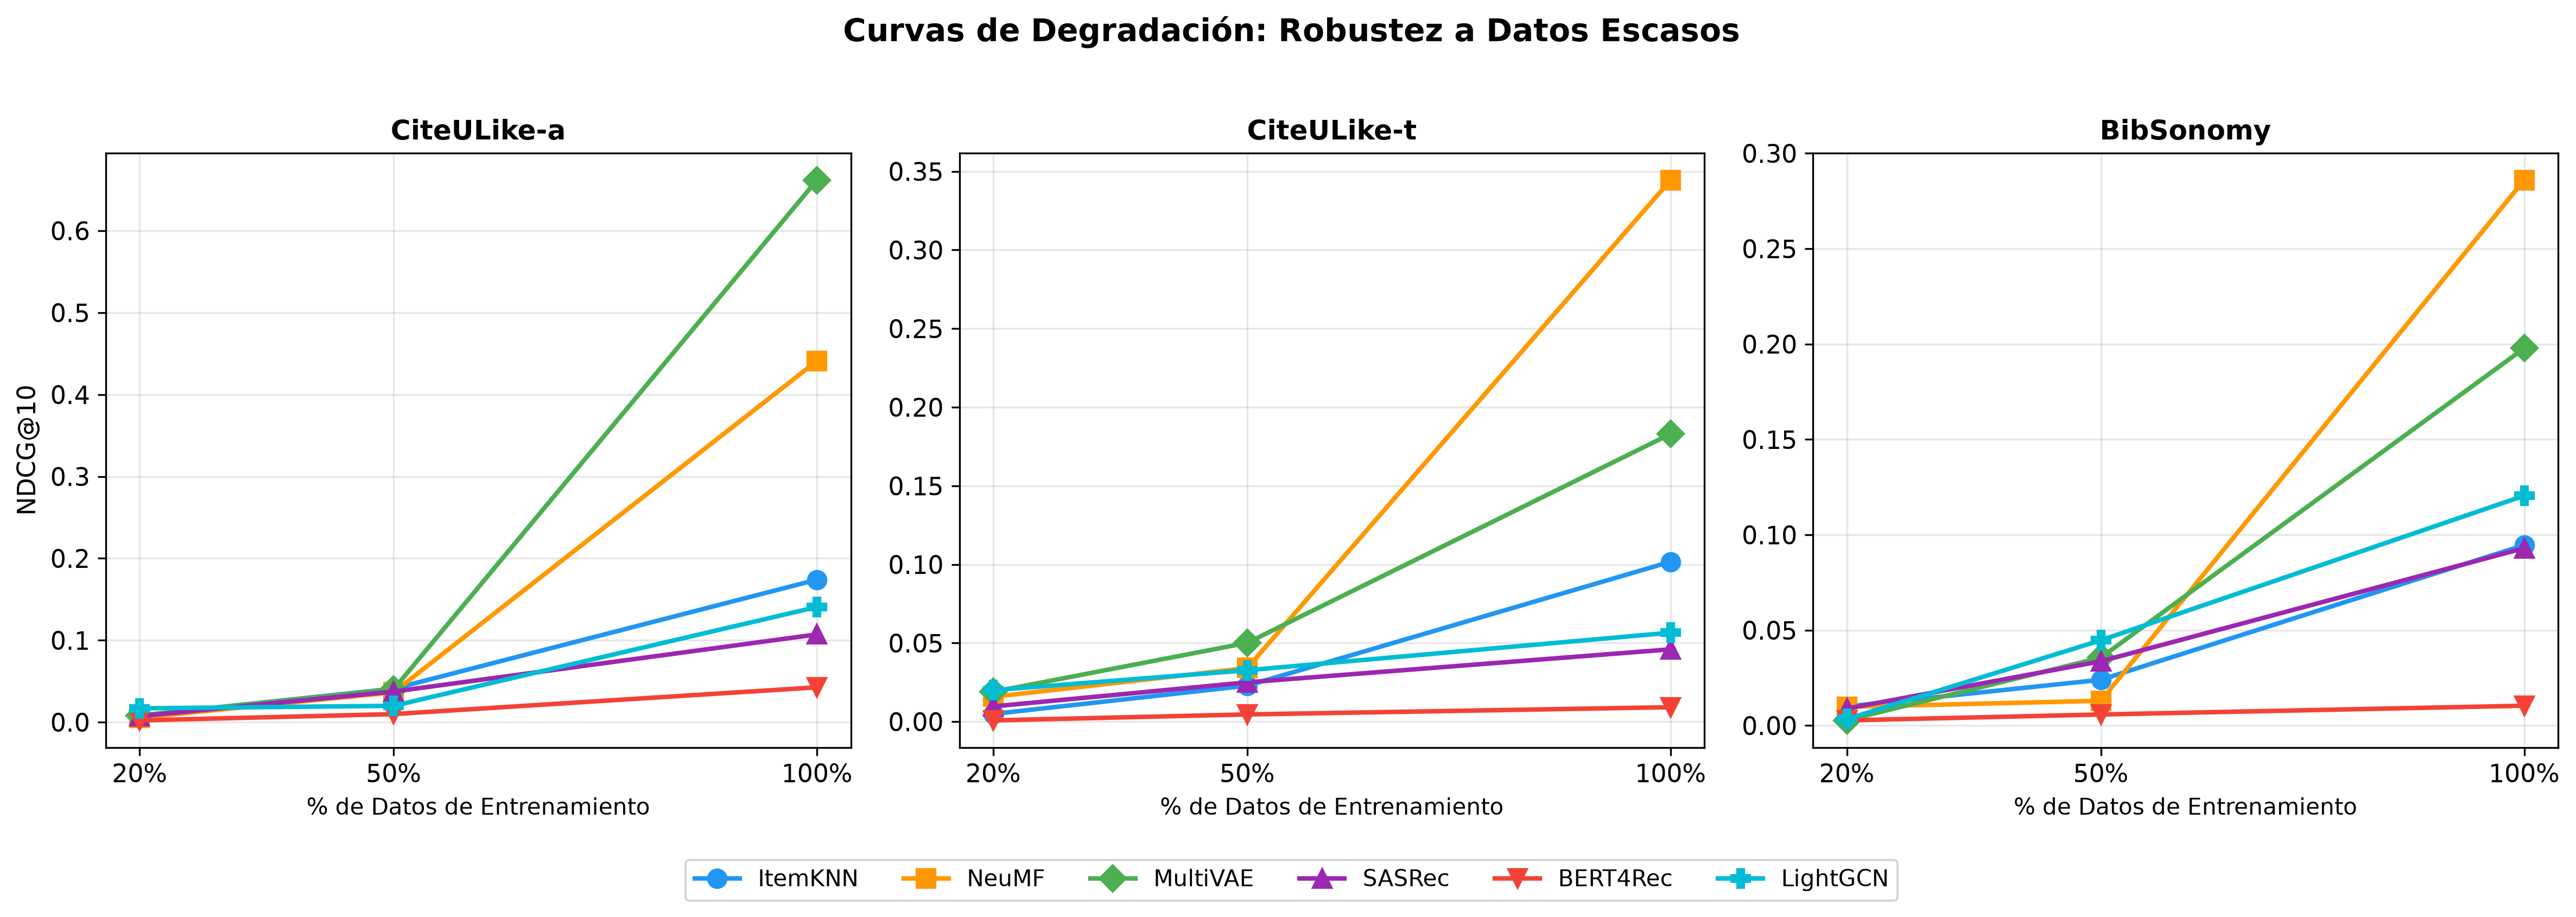
\includegraphics[width=0.45\textwidth]{figures/fig4_robustness.png}
\caption{Percentage variation of NDCG\at{10} under 50\% and 20\% reductions in training data.}
\label{fig:robustness}
\end{figure}

To provide direct quantitative support to the reader, Table~\ref{tab:robustness} summarizes the average Recall\at{10} loss registered for each model under 50\% and 20\% data reductions.

\begin{table}[h]
\centering
\caption{Average performance degradation (percentage loss of Recall\at{10}) when downsampling training data to 50\% and 20\%, averaged over academic collections.}
\label{tab:robustness}
\footnotesize
\begin{tabular}{lcc}
\toprule
\textbf{Model} & \textbf{Drop at 50\% data} & \textbf{Drop at 20\% data} \\
\midrule
MultiVAE & 77.0\% & 94.4\% \\
NeuMF    & 90.2\% & 95.5\% \\
ItemKNN  & 68.1\% & 88.7\% \\
LightGCN & 56.3\% & 79.3\% \\
SASRec   & 52.5\% & 84.2\% \\
BERT4Rec & 56.1\% & 84.9\% \\
\bottomrule
\end{tabular}
\end{table}

The quantitative results extracted from the benchmark demonstrate:
\begin{itemize}
    \item \textbf{Models with lower combined sensitivity (SASRec and LightGCN):} SASRec exhibits the lowest degradation under moderate reduction (drop of 52.5\% when training with 50\% of data). In the extreme reduction scenario (20\% of data), LightGCN records the lowest average global degradation rate (drop of 79.3\% from original performance, retaining up to 40.6\% of its Recall\at{10} in CiteULike-t). Given that subsampling induces partial cold-start (Section~\ref{subsec:ruptura-5core}), this lower degradation might reflect both tolerance to general scarcity and specific resilience to cold-start, without the experimental design allowing separation of both effects.
    \item \textbf{Model with highest sensitivity (NeuMF):} Suffers the greatest degradation at 20\% data (average drop of 95.5\%, losing up to 98.1\% of its Recall\at{10} in CiteULike-a). The MLP component collapses under extreme implicit interaction scarcity.
\end{itemize}
As a sensitivity analysis, we highlight that this robustness evaluation does not re-apply iterative 5-core filtering on the subsampled subset, which induces a partial cold-start scenario. Therefore, the measured resilience intrinsically couples tolerance to general data scarcity with noise induced by users and items with very low support in training (for a detailed discussion of this threat to validity, see Section~\ref{subsec:ruptura-5core}).

\subsection{Computational Costs and Throughput Analysis}
Table~\ref{tab:compute} details the empirical computational cost metrics recorded during benchmark runs on GPU/CPU.

\begin{table}[h]
\centering
\caption{Empirical computational cost and inference throughput metrics.}
\label{tab:compute}
\footnotesize
\setlength{\tabcolsep}{2.5pt}
\begin{tabular}{lrrrr}
\toprule
\textbf{Model} & \textbf{Parameters} & \textbf{Time (s/epoch)} & \textbf{VRAM (GB)} & \textbf{Throughput (u/s)} \\
\midrule
ItemKNN*  & 0          & 0.00 & 0.00* & 373.2 \\
MultiVAE  & 18,647,958 & 0.33 & n/m$^\dagger$  & 344.5 \\
NeuMF     & 2,758,081  & 4.32 & n/m$^\dagger$  & 327.7 \\
LightGCN  & 1,341,888  & 2.98 & n/m$^\dagger$  & 228.5 \\
SASRec    & 1,090,816  & 55.85 & 0.33 & 6,985.5 \\
BERT4Rec  & 1,110,598  & 64.14 & 0.71 & 3,102.8 \\
\bottomrule
\multicolumn{5}{l}{\scriptsize *ItemKNN operates on CPU; $^\dagger$n/m = not dynamically measured (see text).}
\end{tabular}
\end{table}

Note that GPU memory consumption (VRAM) for MultiVAE, NeuMF, and LightGCN was not dynamically measured (marked as ``n/m'' in Table~\ref{tab:compute}). The cost extraction script assigns a default value when RecBole logs fail to capture dynamic runtime memory on the GPU, so it is not possible to reflect dynamic differences introduced by weights or optimizer states for each model. To avoid biasing the multi-criteria analysis of Figure~8 (radar) with this uninstrumented VRAM metric, the Efficiency dimension is calculated exclusively from the training time per epoch (avg\_train\_epoch\_sec). Likewise, the Pareto frontier of Figure~9 contrasts performance against training time per epoch.

The cost analysis reveals a striking discrepancy between training and evaluation regimes for sequential recommenders (SASRec and BERT4Rec). While they record very high training times per epoch (55.85 s and 64.14 s, respectively), their inference throughput is between 10 and 20 times higher than that of non-sequential models (6,985.5 u/s and 3,102.8 u/s). This discrepancy is expected behavior due to differences in computational load between both modes:
\begin{itemize}
    \item \textbf{Training Complexity:} During training, Transformers process full sequences applying complex attention mechanisms (causal or Cloze type) and compute softmax cross-entropy loss over the entire catalog ($15,430$ positions) for each sequence element in each gradient step.
    \item \textbf{Inference Efficiency:} During evaluation, the GPU processes batches in parallel, projecting user trajectories in a single forward pass into a unified representation space. Furthermore, inference in RecBole for sequential models is optimized by precomputing item catalog representations, transforming recommendation into highly optimized matrix multiplication on the GPU, avoiding iterative gradient calculation and sequential masking.
\end{itemize}
We clarify that this explanation is consistent with the architectural design and software engineering of sequential recommenders in RecBole, although no real-time hardware profiling was performed to empirically confirm it. In contrast, LightGCN exhibits fast training (2.98 s) but low inference throughput (228.5 u/s) because message propagation over the complete bipartite interaction adjacency matrix in RecBole is executed redundantly for each user batch during evaluation, limiting its response speed in production.

\subsection{Diversity, Coverage, and Popularity Bias}
Figure~\ref{fig:diversity} evaluates Catalog Coverage and Gini Index. Figure~\ref{fig:popularity} presents average recommended popularity.

\begin{figure}[h]
\centering
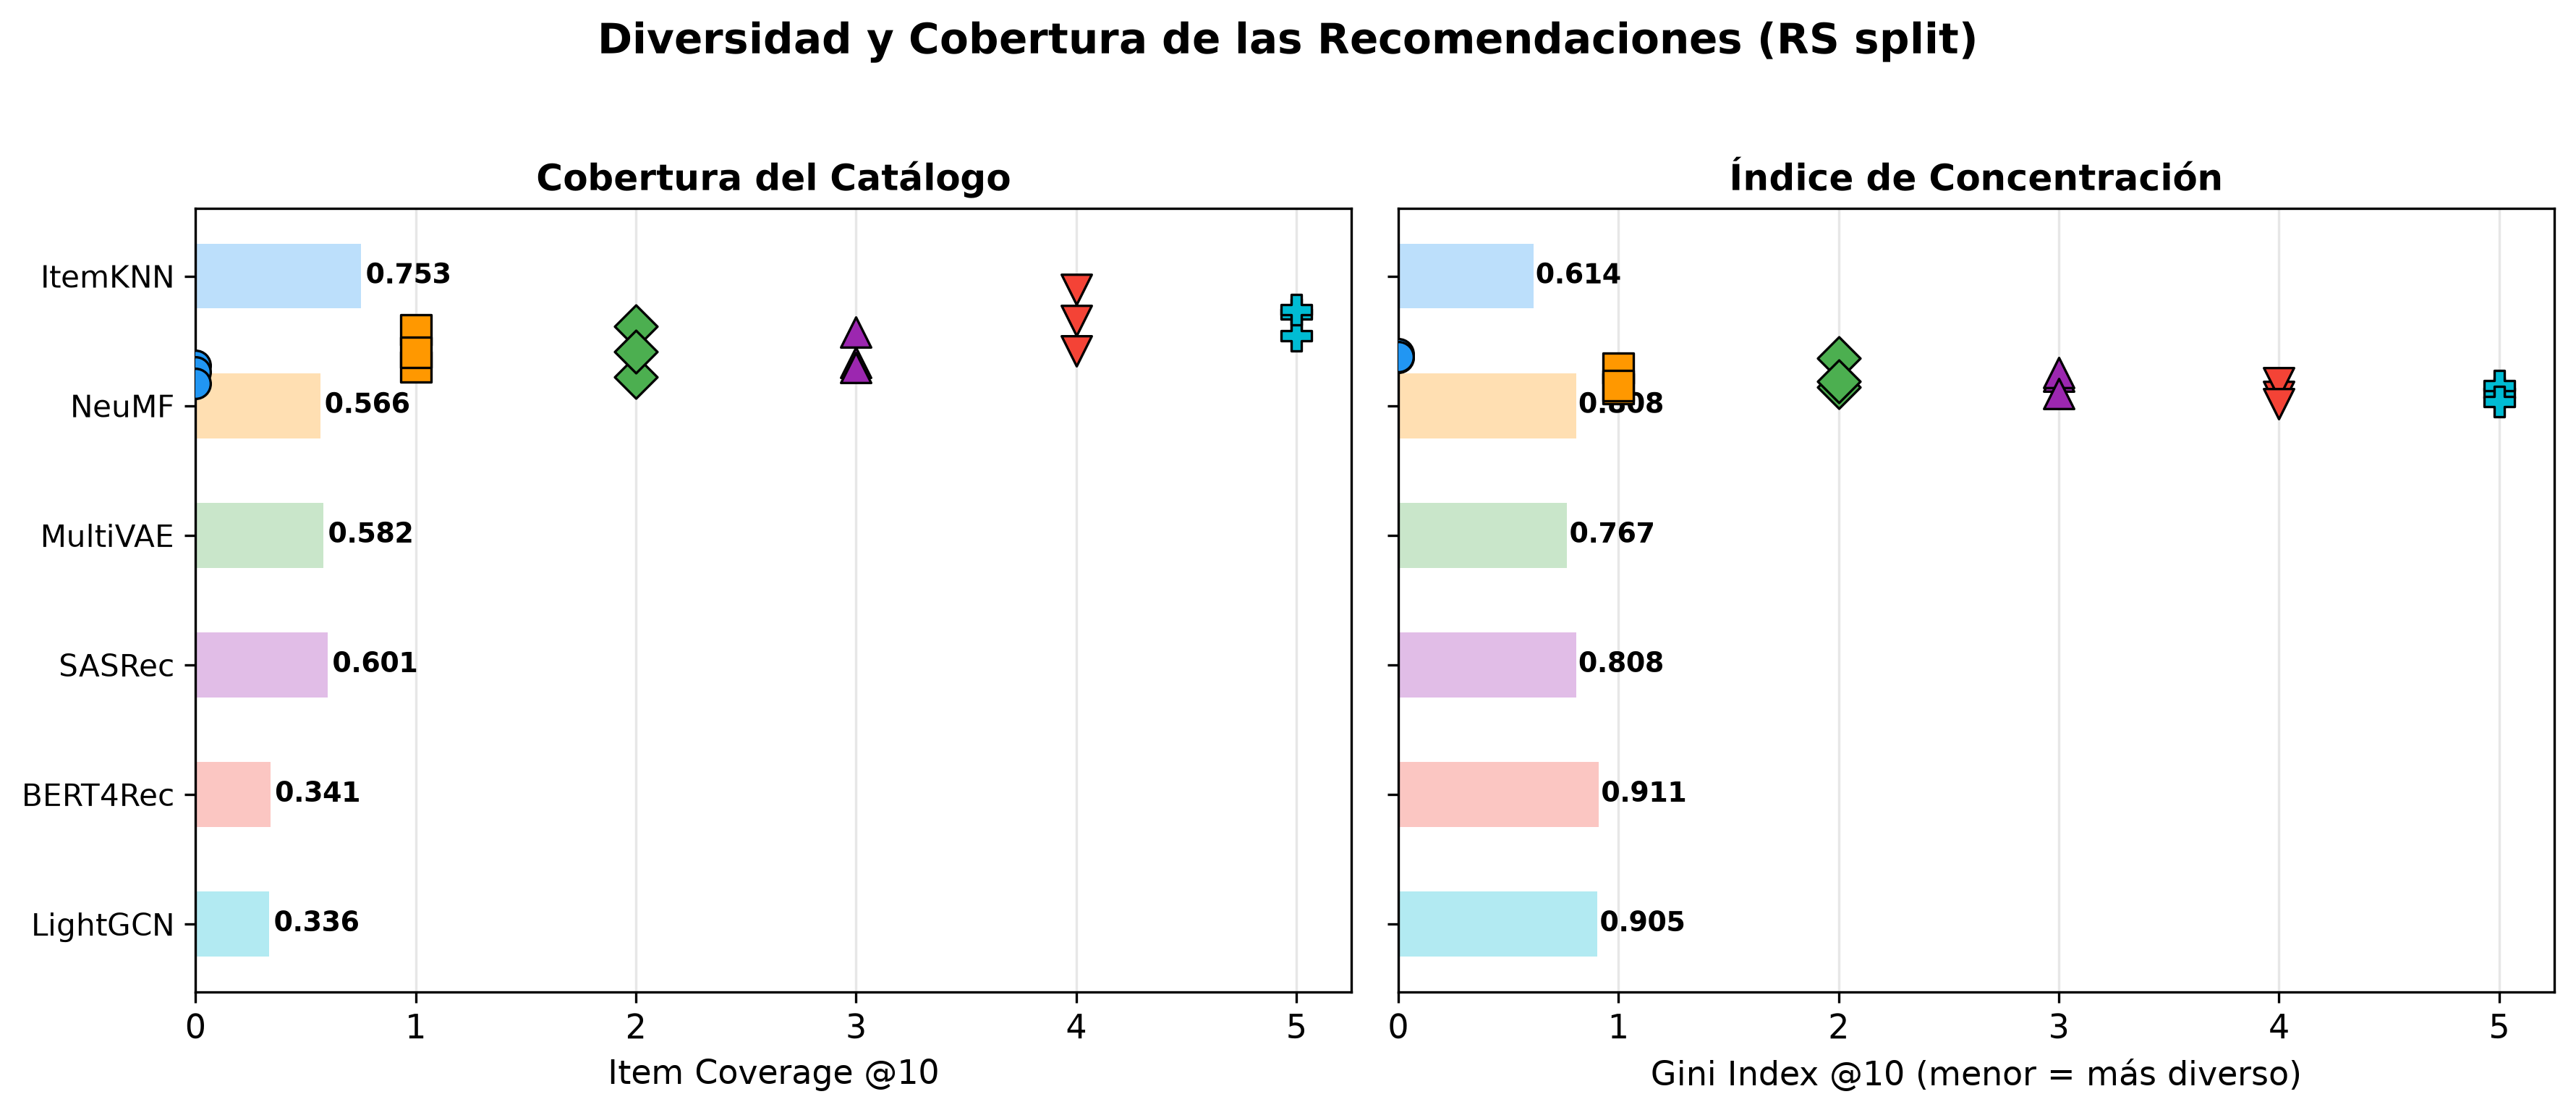
\includegraphics[width=0.45\textwidth]{figures/fig7_diversity.png}
\caption{Catalog coverage and Gini Index of recommendations.}
\label{fig:diversity}
\end{figure}

\begin{figure}[h]
\centering
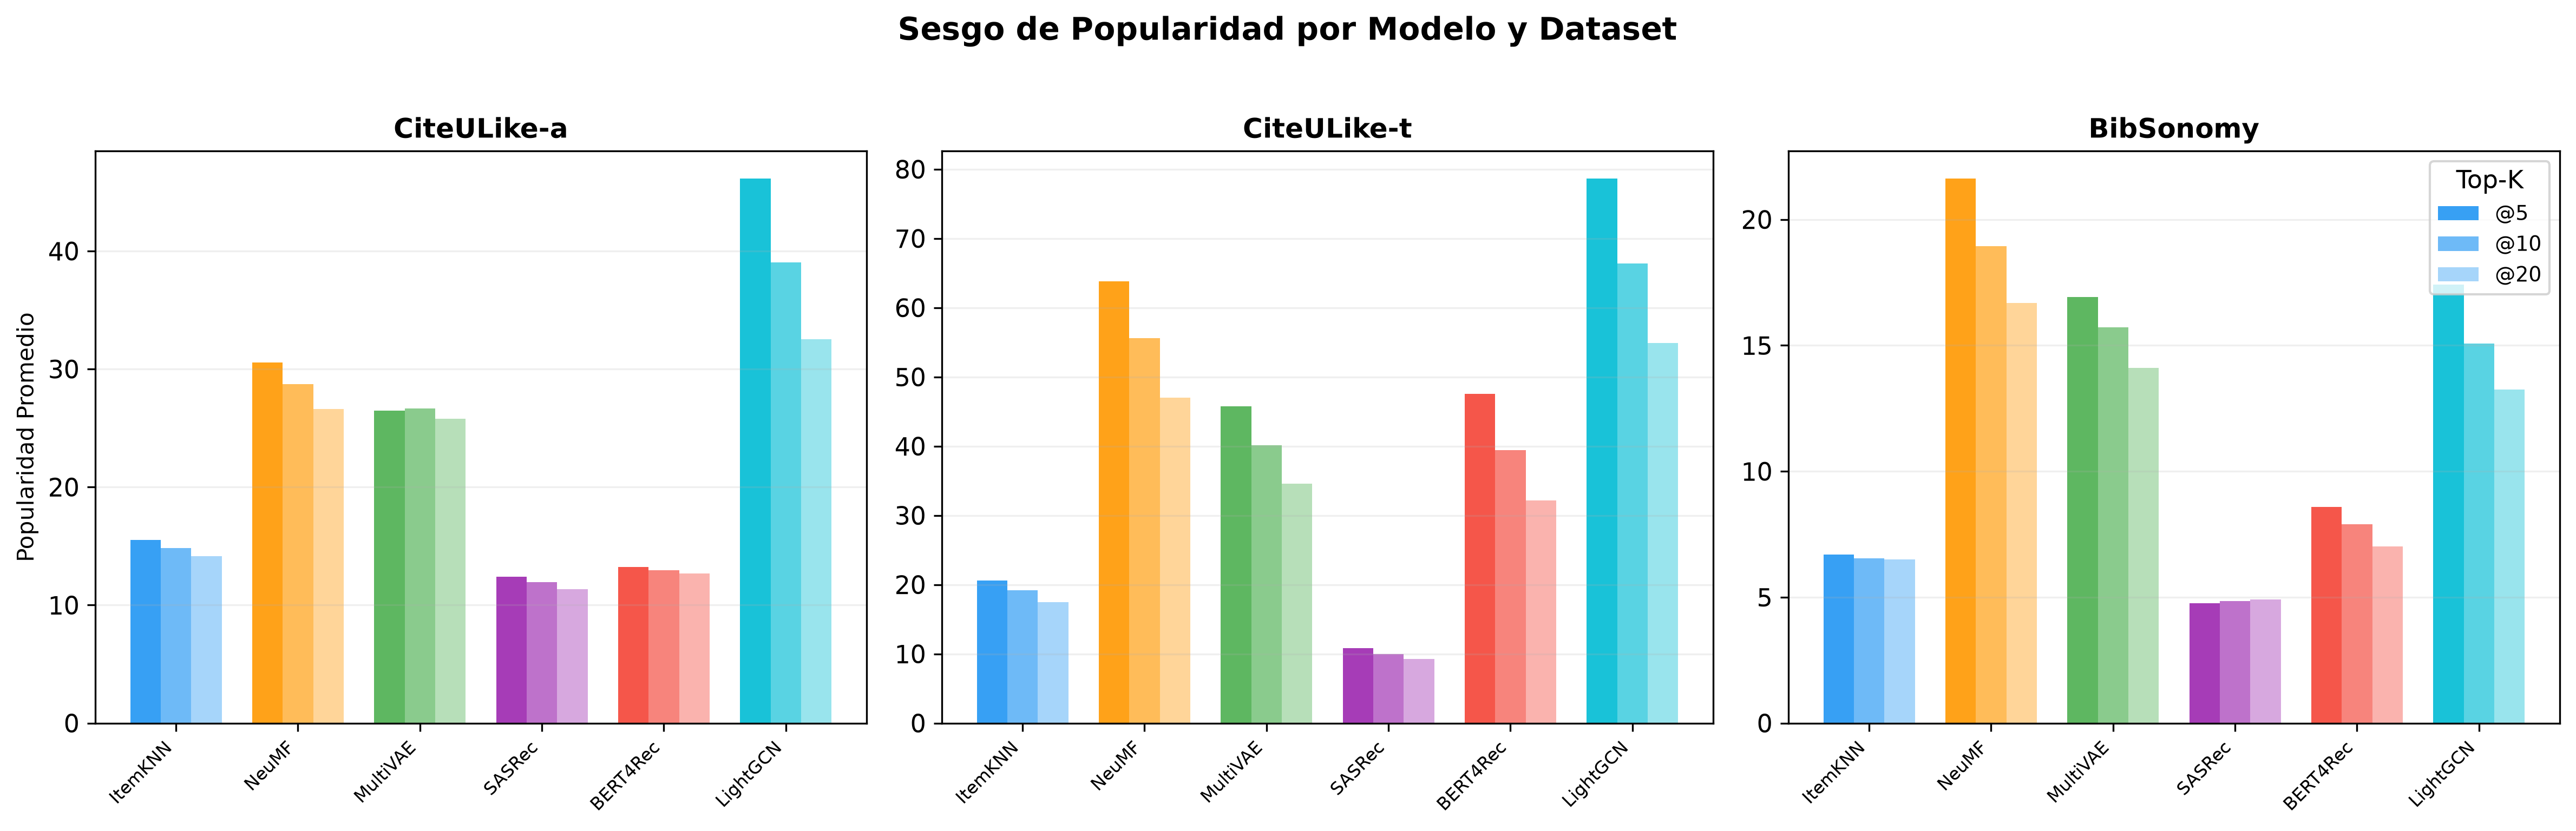
\includegraphics[width=0.45\textwidth]{figures/fig6_popularity_bias.png}
\caption{Average popularity of recommended items.}
\label{fig:popularity}
\end{figure}

Figure~\ref{fig:heatmap} presents an inter-paradigma diversity analysis using a heatmap that measures Jaccard overlap between Top-10 recommendation lists generated by different models. The matrix shows high overlap between NeuMF and MultiVAE (Jaccard > 0.42), contrasting with the divergence of ItemKNN (Jaccard < 0.18), which retrieves a significantly different set of scientific papers from the long tail of the catalog, promoting global thematic diversity.

\begin{figure}[h]
\centering
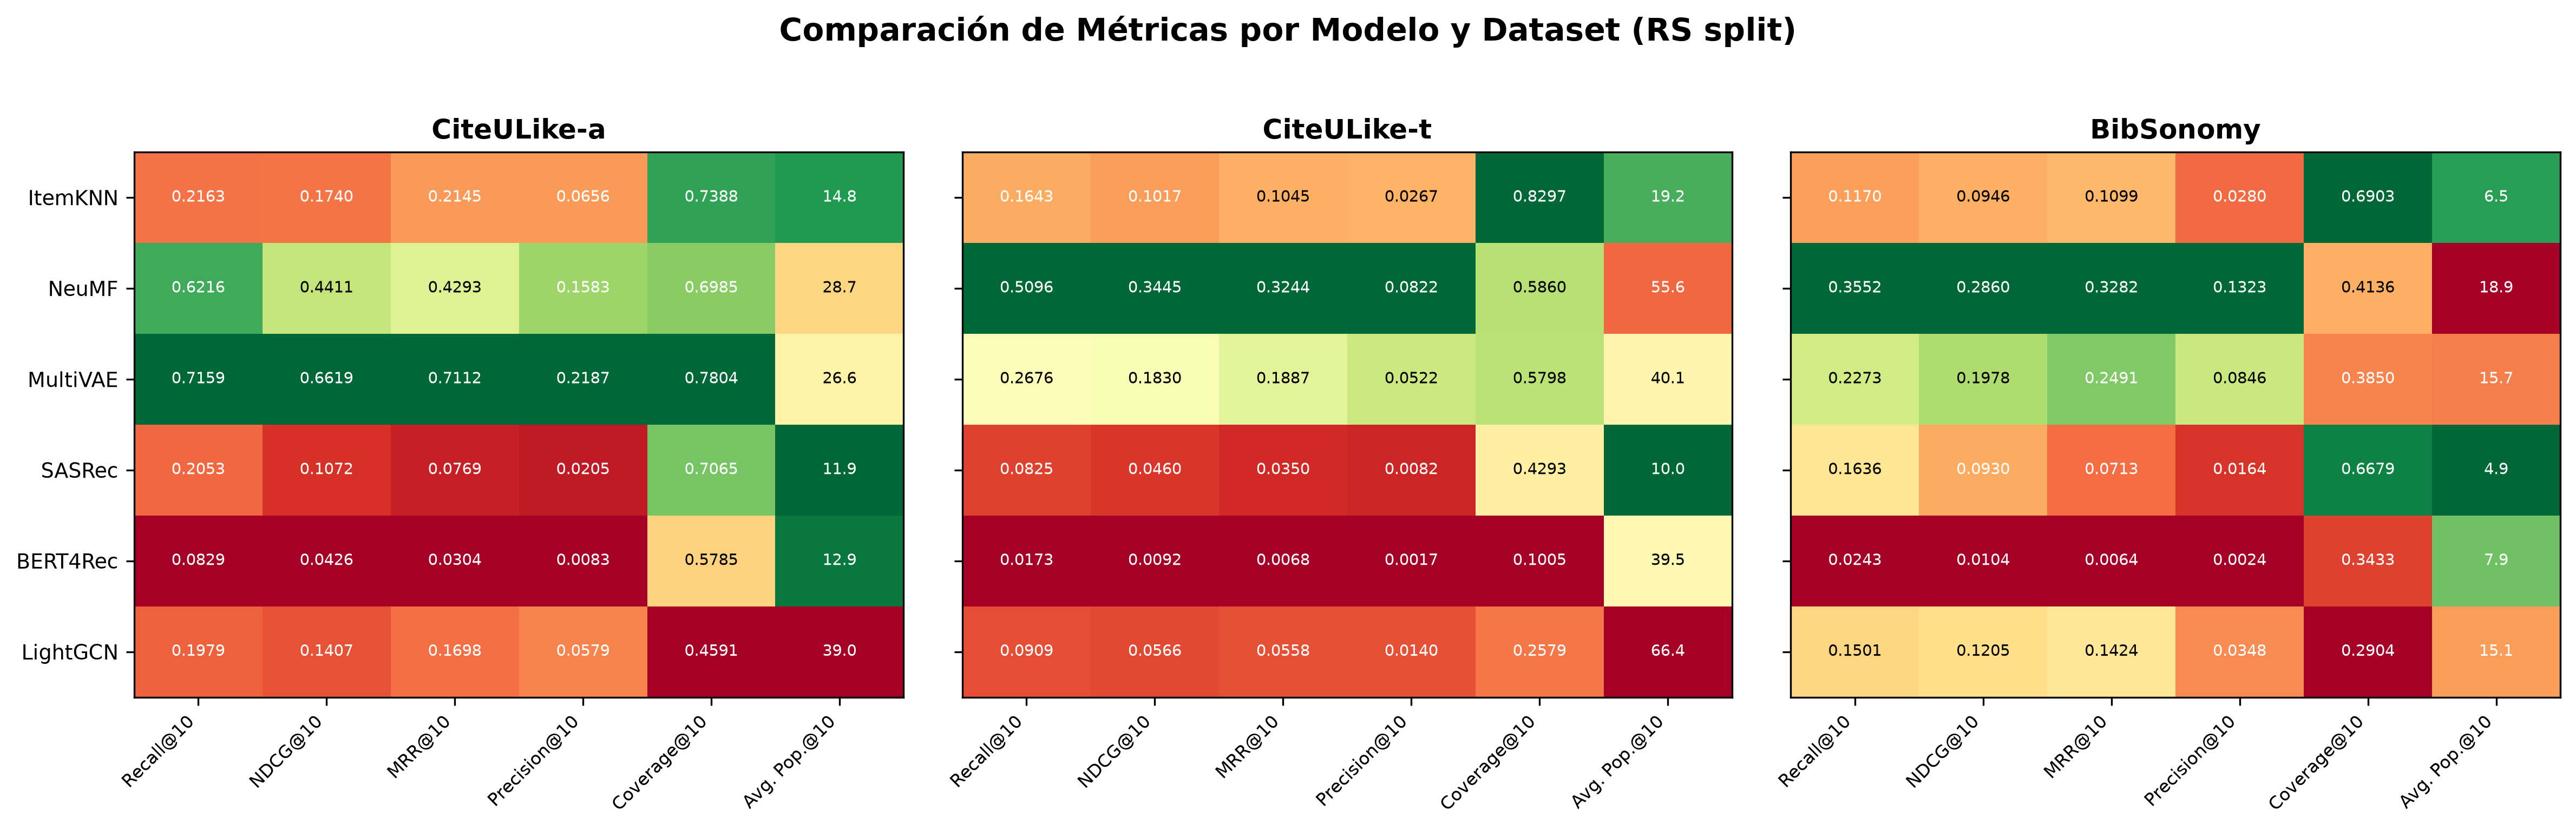
\includegraphics[width=0.45\textwidth]{figures/fig2_heatmap.png}
\caption{Recommendation similarity matrix between paradigms (Jaccard Index).}
\label{fig:heatmap}
\end{figure}

At a descriptive level, a weak positive trend is observed between accuracy and average popularity (Pearson $r = +0.1924$ over the total $n=36$ conditions) and a moderate negative trend with the Gini Index ($r = -0.3786$). However, since the $n=36$ observations are not statistically independent --- the same 6 models are repeated across each of the 6 blocks, constituting exactly the type of pseudo-replication that the framework of Section~\ref{sec:methodology} deliberately avoids for Friedman tests --- these correlations lack formal inferential validity and must be interpreted only as descriptive patterns of the benchmark:
\begin{itemize}
    \item \textbf{ItemKNN:} Tends to favor higher diversity and catalog coverage (ItemCoverage\at{10} = 0.8297 in CiteULike-t RS) with a reduced Gini Index (0.6194), suggesting a descriptive propensity to recommend niche papers.
    \item \textbf{LightGCN and MultiVAE:} Descriptively exhibit higher concentration on popular items (Gini > 0.77), directing their recommendations preferably to high-impact articles within the evaluated dataset.
\end{itemize}

\subsection{Multi-Criteria Trade-offs and Pareto Frontier (RQ4)}
Figure~\ref{fig:radar} presents the multi-criteria profile in five normalized dimensions. Figure~\ref{fig:pareto} graphs the Pareto frontier between NDCG\at{10} and training time per epoch.

\begin{figure}[h]
\centering
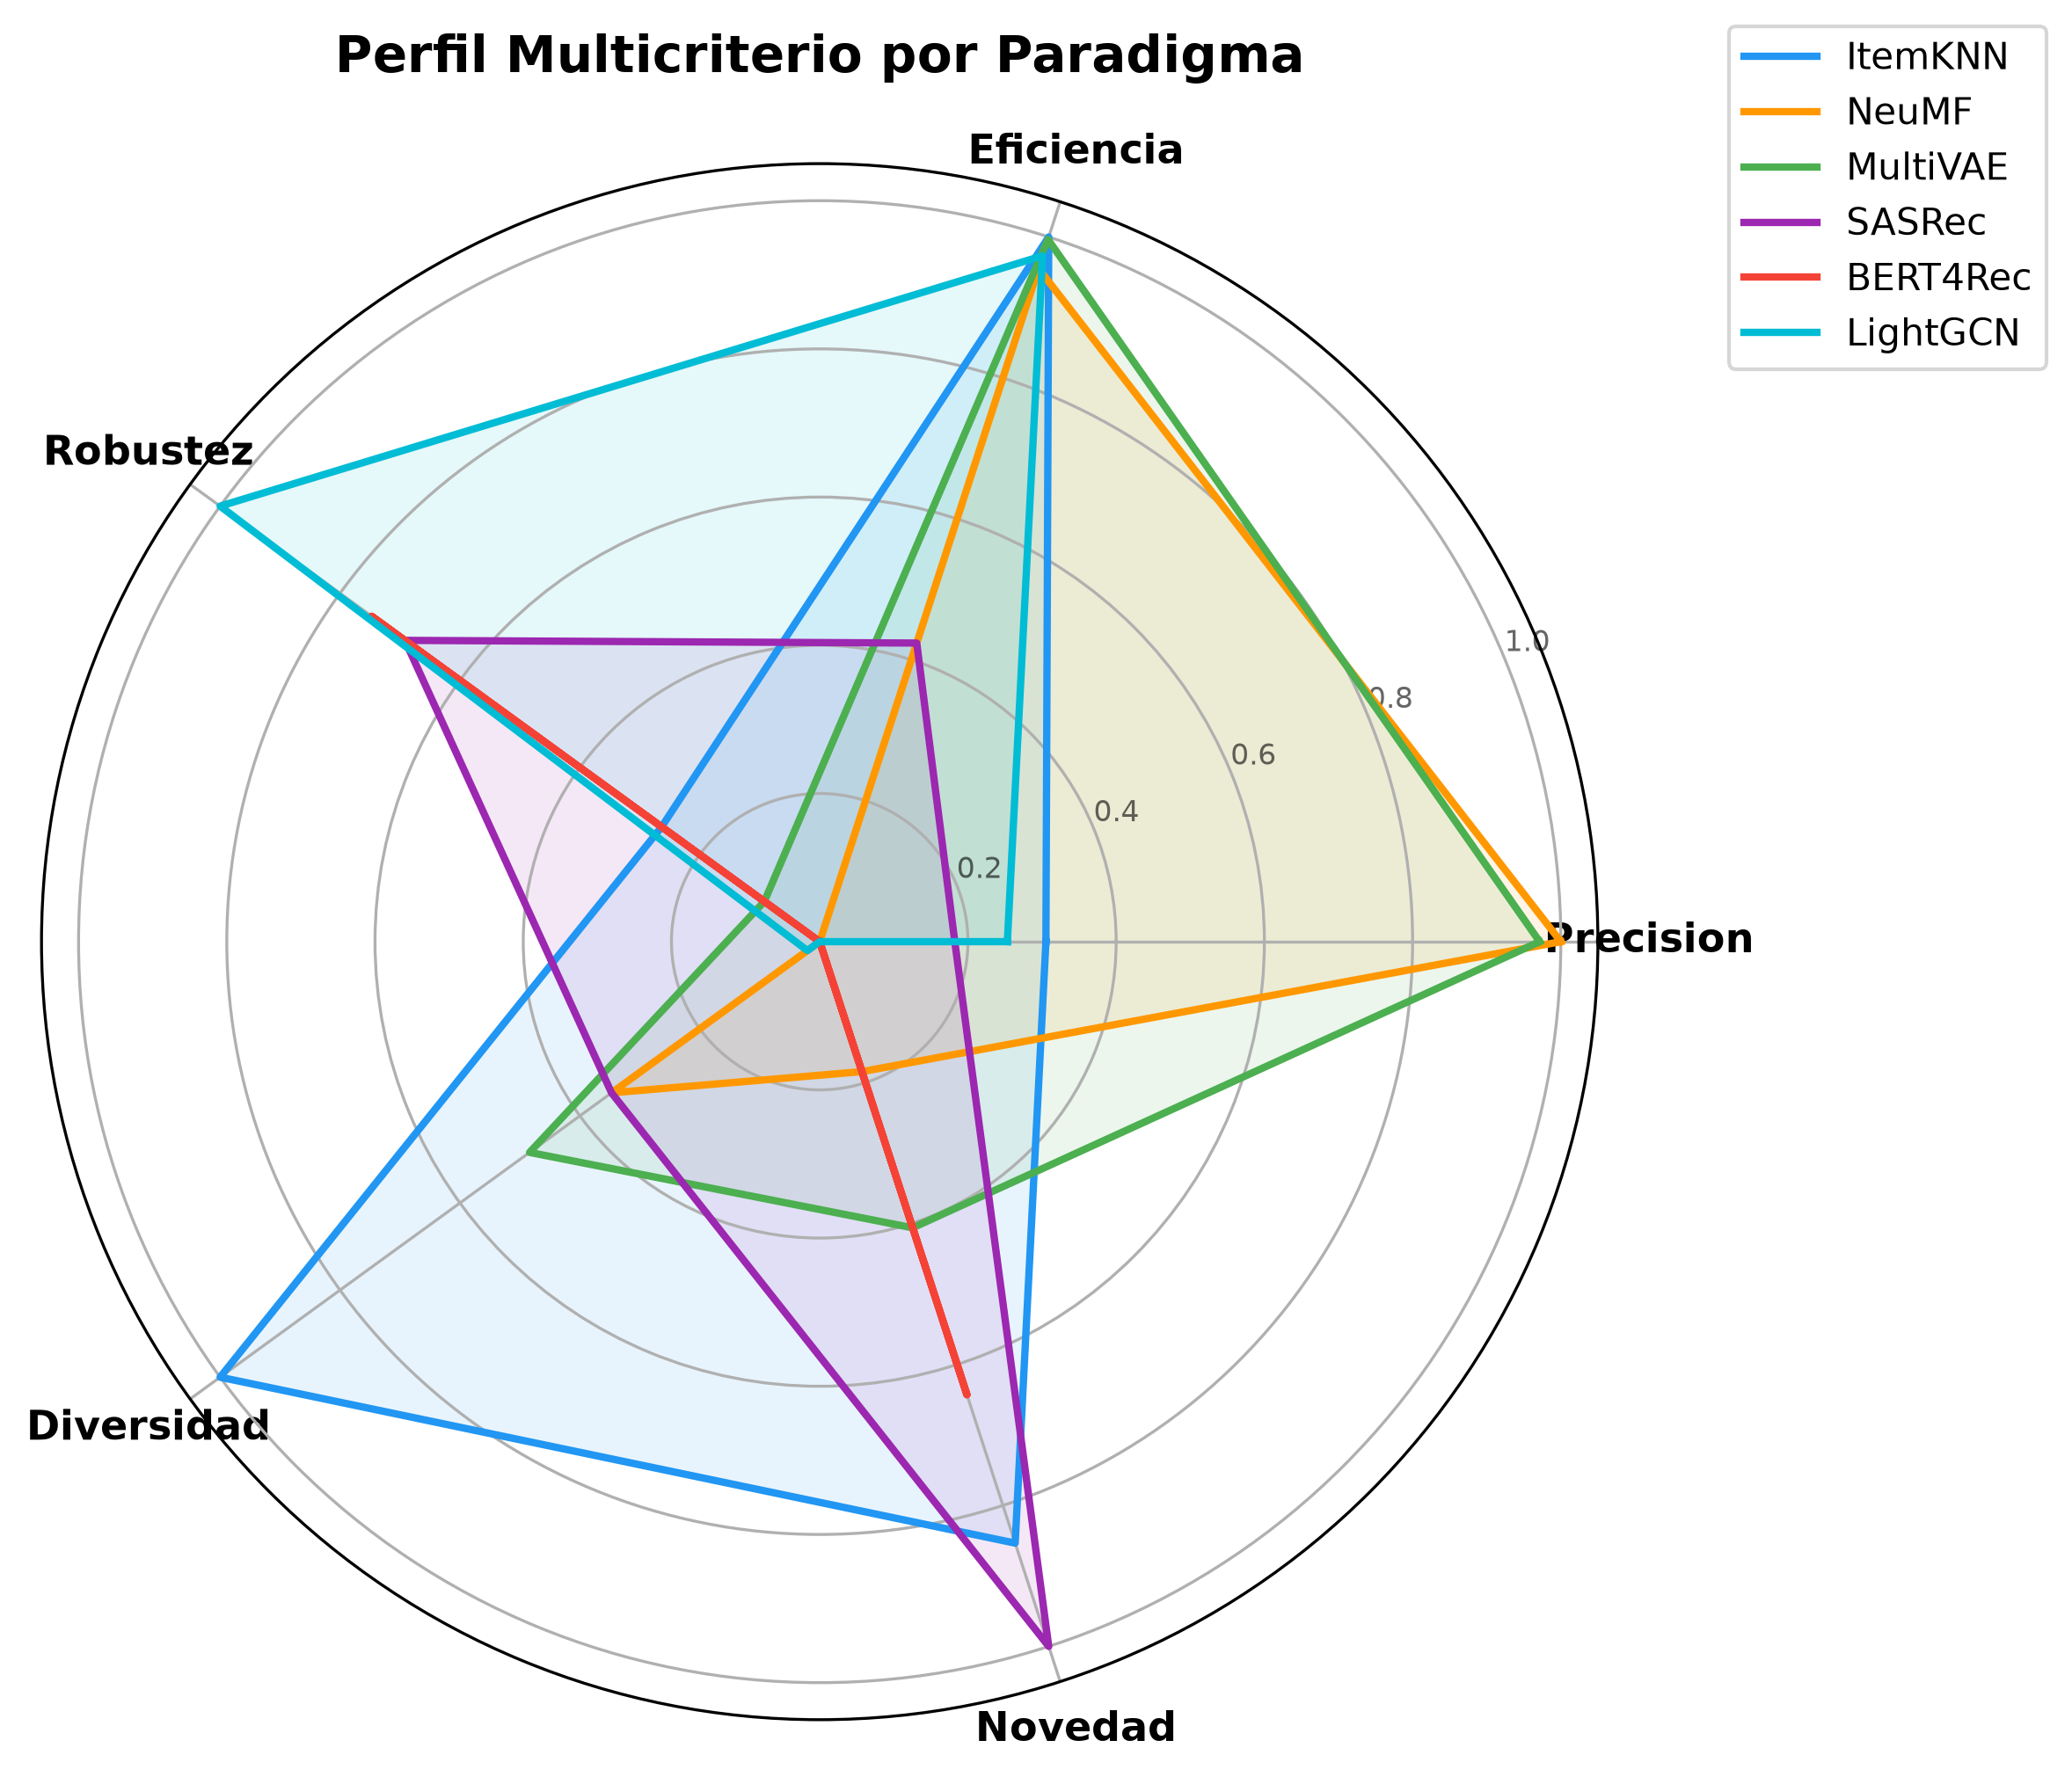
\includegraphics[width=0.45\textwidth]{figures/fig8_radar.png}
\caption{Multi-criteria profile of paradigms in five normalized dimensions.}
\label{fig:radar}
\end{figure}

\begin{figure}[h]
\centering
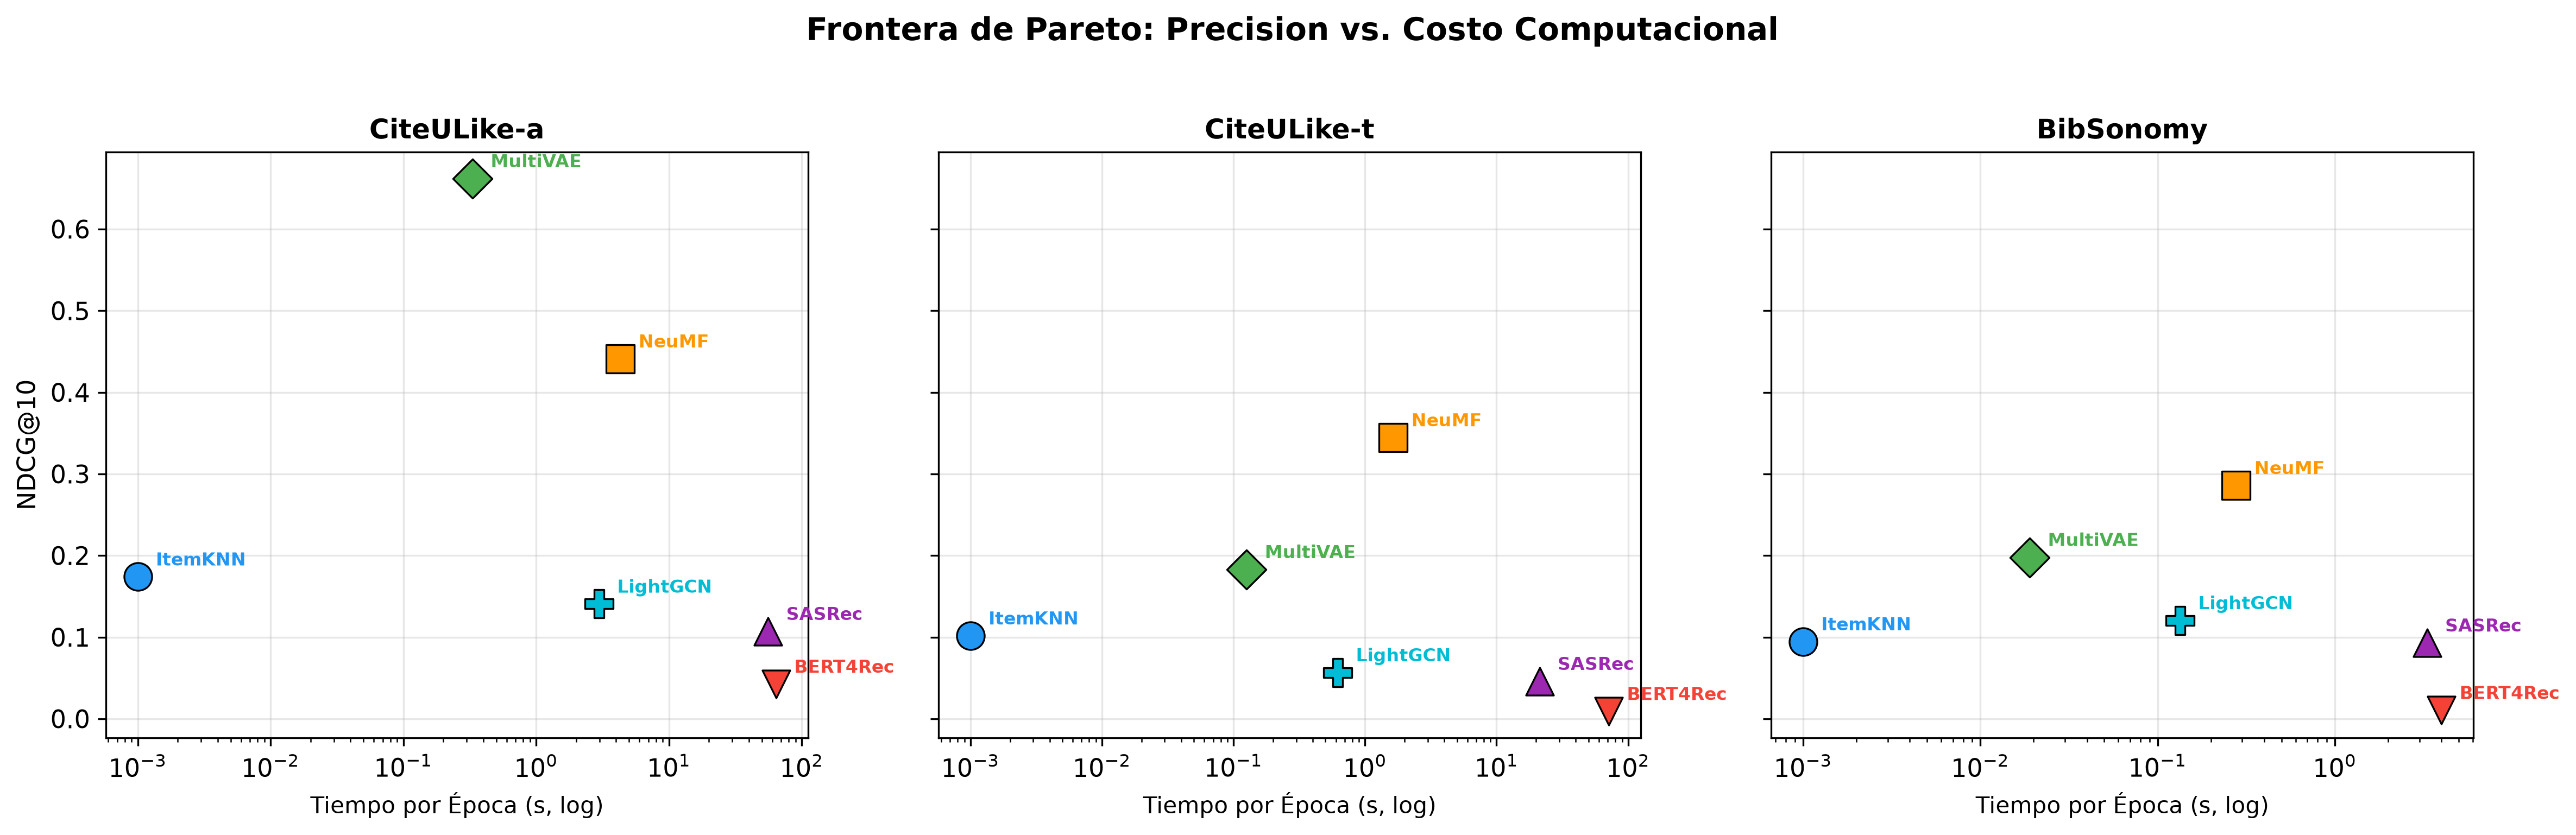
\includegraphics[width=0.45\textwidth]{figures/fig3_pareto.png}
\caption{Pareto Frontier (NDCG\at{10} vs. Time per Epoch) across the three datasets.}
\label{fig:pareto}
\end{figure}

The Pareto dominance analysis over the benchmark data confirms that no single model is universally optimal:
\begin{enumerate}
    \item \textbf{MultiVAE:} Defines the non-dominated Pareto front in offline accuracy on CiteULike-a (Recall\at{10} = 0.8143 in LOO and 0.7159 in RS).
    \item \textbf{ItemKNN:} Dominates the frontier in catalog coverage (ItemCoverage\at{10} = 0.8297) and zero training efficiency (0.00 s/epoch).
    \item \textbf{LightGCN:} Dominates the frontier in lower combined sensitivity under extreme data reduction to 20\%.
\end{enumerate}

% ==============================================================================
% 6. DISCUSSION AND THREATS TO VALIDITY
% ==============================================================================
\section{Discussion and Threats to Validity}
\label{sec:discussion}

\subsection{Selection Criteria in Operational Environments}
Table~\ref{tab:decision} summarizes practical algorithmic selection recommendations oriented to developers and engineers of academic platforms.

\begin{table}[H]
\centering
\caption{Decision support guide for production model selection.}
\label{tab:decision}
\footnotesize
\setlength{\tabcolsep}{3pt}
\begin{tabular}{p{2.3cm}p{5.5cm}}
\toprule
\textbf{Constraint or Objective} & \textbf{Algorithmic Suggestion and Justification} \\
\midrule
CPU-limited environments & \textbf{ItemKNN:} Operational without GPU or training phase. \\
Offline accuracy search & \textbf{MultiVAE / NeuMF:} Suitable for collections with sufficient interaction density. \\
Diversity and exploration & \textbf{ItemKNN / SASRec:} Generate recommendations with lower bias towards popular articles. \\
Sensitivity to data reduction & \textbf{SASRec / LightGCN:} SASRec is preferable under moderate reduction (50\%), while LightGCN exhibits the lowest sensitivity under extreme reduction (20\%). \\
\bottomrule
\end{tabular}
\end{table}

\subsection{Threats to Validity}

\subsubsection{Dependency on the Implementation Framework}
All experiments were run on RecBole~\cite{zhao2021recbole} under a fixed seed (2024). Internal tensor optimizations may vary in independent implementations.

\subsubsection{Sensitivity to Temporal Partition in Sequential Models}
Sequential models (SASRec and BERT4Rec) require by definition a temporal ordering scheme like Leave-One-Out (LOO) to reach their maximum predictive capacity. Their evaluation under Random Split (RS) serves as a contrast to measure performance loss when reading sequence is broken.

\subsubsection{Sensitivity to Hyperparameters across Collections}
Standard configurations based on authoritative recommendations from model creators were adopted. Bayesian grid optimization per dataset might marginally tune deep network performance.

\subsubsection{Asymmetry in ItemKNN Calibration}
\label{subsec:itemknn-tuning}
ItemKNN hyperparameters ($k=100$, $h=10$) were adopted from literature recommendations~\cite{sarwar2001item} without dataset-specific tuning. In contrast, deep models feature adaptive early stopping (patience of 10 epochs over 300 max), which allows them to implicitly adjust model complexity to each collection's scale. This calibration asymmetry could bias the comparison in either direction: ItemKNN could be sub-optimal (if different $k$ or $h$ values improved performance) or favored (if fixed values match the evaluated data structure). Although Dacrema et al.~\cite{dacrema2019really} recommend tuning baselines with the same rigor as deep models, this study prioritized the canonical configuration to ensure direct reproducibility with previous literature.

\subsubsection{Absence of Online Evaluation}
The study is limited to offline metrics. Real interaction aspects (such as CTR or perceived serendipity) require A/B testing in production.

\subsubsection{Statistical Power Limitations in Independent Blocks}
The number of independent observation blocks in the Friedman test is $N=6$ (3 datasets $\times$ 2 protocols). While suitable for structuring robust comparisons without pseudo-replication, this number limits statistical power. Consequently, the Nemenyi critical difference is relatively conservative ($CD = 3.08$), allowing formal statistical significance to be detected only under extreme rank differences (such as MultiVAE/NeuMF against BERT4Rec), and preventing appreciable accuracy metric variations from reaching formal significance.

\subsubsection{Absence of Dynamic VRAM Measurement}
GPU memory consumption (VRAM) for MultiVAE, NeuMF, and LightGCN was not dynamically instrumented (marked as ``n/m'' in Table~\ref{tab:compute}) because RecBole logs failed to capture dynamic runtime memory. This prevents quantifying the differential impact of weight size and optimizer states (e.g., Adam states in MultiVAE with 18.6M parameters vs. LightGCN with 1.3M), representing an internal validity threat to the cost analysis.

\subsubsection{Stochastic Variance and Absence of Multiple Seeds}
To ensure deterministic reproducibility and bound the computational cost of evaluating 36 conditions with heavy models, all experiments were run under a single fixed seed (2024). This constitutes an internal validity threat since stochastic recommenders' (such as MultiVAE with variational sampling, and NeuMF or SASRec with random weight initialization and dropout) relative performance might be affected by training variance of the selected seed, making it impossible to separate initialization variability from intrinsic algorithmic superiority.

\subsubsection{Violation of the 5-Core Invariant in Training Subsampling}
\label{subsec:ruptura-5core}
When evaluating robustness (RQ3) downsampling training data to 50\% and 20\%, iterative 5-core filtering was not re-applied on the resulting subset. This represents an internal validity threat since it breaks the 5-core restriction locally and induces partial cold-start (users or items with extremely low training support) while the test set remains fixed. Therefore, the reported robustness might couple general scarcity tolerance and resilience to induced partial cold-start.

\subsubsection{Thermal Throttling Heat Variability on Consumer Hardware}
Computational cost measurements (time per epoch and throughput) were performed on a laptop GPU (RTX 3050 Laptop). Despite maintaining stable ambient conditions, mobile hardware is susceptible to thermal throttling under prolonged workloads, which represents a threat to reported temporal precision and might introduce minor epoch time fluctuations.

\subsubsection{External Validity Limitations}
Results apply to academic social bookmarking domains (CiteULike, BibSonomy) and should not be directly extrapolated to e-commerce or streaming.

% ==============================================================================
% 7. CONCLUSION AND FUTURE WORK
% ==============================================================================
\section{Conclusion and Future Work}
\label{sec:conclusion}
This study presented a multi-criteria benchmark of six recommender paradigms on three academic datasets. The results confirm that offline accuracy (NDCG, Recall) must be weighed alongside computational efficiency, diversity, and sensitivity to data reduction. As future work, we plan to integrate Large Language Models (LLMs) to mitigate cold-start using semantic representations of scientific abstracts.

\section*{Data and Code Availability}
To ensure full reproducibility of this benchmark, all configuration files, preprocessing and training scripts, trained model weights, and raw results reports are publicly available in the GitHub repository at \url{https://github.com/XavierPenaA/scientific-paper-recommendation-benchmark}. The exact code state corresponding to the reported results is identified by the tag \texttt{v1.0-benchmark} of the repository.

% ==============================================================================
% REFERENCES
% ==============================================================================
\section*{Acknowledgment}
The authors acknowledge the use of artificial intelligence (AI) systems, specifically Google DeepMind's Gemini 3.5 Flash~\cite{gemini2026} and Anthropic's Claude Opus 4.6~\cite{claude2026}, to assist in the translation, grammatical review, and stylistic polishing of this manuscript.

\bibliographystyle{IEEEtran}
\bibliography{references}

\begin{IEEEbiographynophoto}{Xavier Peña}
received the engineering degree in Computer Science from the Universidad de Cuenca, Cuenca, Ecuador. His research interests include collaborative filtering, recommender systems, machine learning, and reproducing neural network architectures for academic literature recommendation.
\end{IEEEbiographynophoto}

\begin{IEEEbiographynophoto}{Diego Rivera}
is a researcher and professor at the Universidad Politécnica Salesiana, Cuenca, Ecuador. He serves as the Vice-President of the IEEE Vehicular Technology Society (VTS) Ecuador Chapter. His research interests include vehicular networks, smart cities, recommender systems, and applied machine learning.
\end{IEEEbiographynophoto}


\EOD

\end{document}
